\documentclass[12pt,a4paper,twoside]{report}

\usepackage[colorlinks,linkcolor=black,urlcolor=black]{hyperref}
\usepackage{amsmath,amssymb,amsthm}
\usepackage[utf8]{inputenc}
\usepackage{xcolor}
\usepackage{xparse}
\usepackage{style}
\usepackage[capitalise]{cleveref}
\usepackage{mathtools}
\usepackage[shortlabels]{enumitem}
\usepackage[style=apa, backend=biber]{biblatex}

\usepackage[record,style=alttreegroup,nomain,symbols]{glossaries-extra}

\usepackage{dutchcal} 

\usepackage{pdfpages}

\usepackage[T1]{fontenc}
%%%%%%%%%%%%%%%%
% Seitenlayout %
%%%%%%%%%%%%%%%%

% DIV# gibt den Divisor für die Layoutberechnung an.
% Vergrößern des Divisors vergrößert den Textbereich.
% BCOR#cm gibt die Breite des Bundstegs an.
\usepackage[DIV14,BCOR2cm]{typearea}

% Abstand obere Blattkante zur Kopfzeile ist 2.54cm - 15mm
%\setlength{\topmargin}{-15mm}

% Keine Einrueckung nach einem Absatz.

%\parindent 0pt

% Abstand zwischen zwei Abs\"atzen.

%\parskip 12pt

% Zeilenabstand.

\linespread{1.25}



\usepackage{makeidx}
\makeindex


% \newtheoremstyle{break}%
% {}{}%
% {\itshape}{}%
% {\bfseries}{}% % Note that final punctuation is omitted.
% {\newline}{}
%
% \theoremstyle{break}
% \theoremstyle{plain} 

\newtheoremstyle{mytheoremstyle} % name
    {\topsep}                    % Space above
    {\topsep}                    % Space below
    {\itshape}                   % Body font
    {}                           % Indent amount
    {\bfseries}                  % Theorem head font
    {.}                          % Punctuation after theorem head
    {\newline}                   % Space after theorem head
    {}  % Theorem head spec (can be left empty, meaning ‘normal’)

\theoremstyle{mytheoremstyle}

% \makeatletter
% \def\thmhead#1#2#3{%
%   \thmname{#1}\thmnumber{ #2}\thmnote{ (#3)}% 
%   \newline
% }
% \makeatother
% \renewcommand{\@thmheadpunct}{}

\newtheorem{thm}{Theorem}[section]
\newtheorem{lem}[thm]{Lemma}
\newtheorem*{thm*}{Theorem}
\newtheorem*{lem*}{Lemma}
\newtheorem{cor}[thm]{Corollary}

\newtheoremstyle{mytheoremstyle2} % name
    {\topsep}                    % Space above
    {\topsep}                    % Space below
    {}                           % Body font
    {}                           % Indent amount
    {\bfseries}                  % Theorem head font
    {.}                          % Punctuation after theorem head
    {\newline}                   % Space after theorem head
    {}  % Theorem head spec (can be left empty, meaning ‘normal’)

\theoremstyle{mytheoremstyle2}

\newtheorem{defi}[thm]{Definition}
\newtheorem{ax}[thm]{Axiom}
\newtheorem{ex}[thm]{Example}

\newtheorem{proofpart}{Part}
\makeatletter
\@addtoreset{proofpart}{thm}
\makeatother

\newtheorem{proofpp}{Subpart}[proofpart]



\theoremstyle{remark}
\newtheorem{rem}[thm]{Remark}
\newtheorem*{rem*}{Remark}


% \DeclareOldFontCommand{\sc}{\normalfont\scshape}{\@nomath\sc}

% \expandafter\def\expandafter\normalsize\expandafter{%
%     \normalsize%
%     \setlength\abovedisplayskip{0pt}%
%     \setlength\belowdisplayskip{8pt}%
%     \setlength\abovedisplayshortskip{-8pt}%
%     \setlength\belowdisplayshortskip{2pt}%
% }

\newenvironment{sourcescontribs}{%
  \section*{Sources and Original Contributions}%
}{}


\makeglossaries

\setglossarypreamble{
  This list of acronyms only specifies the most important ones
  %TODO: write glossary intro
}

%   PS_Metrics
\newglossaryentry{metric}{name={\ensuremath{\metric}}, description={A metric function. Depending on the context, this refers to an arbitrary metric, or the metric from the segmentally additive AD model}, text={}}

\newglossaryentry{metricSpace}{name={\ensuremath{\langle X, \metric \rangle}}, description={A metric space}, text={}}

\newglossaryentry{PS}{
  name={\ensuremath{\langle \ps{A}, \succsim \rangle}},
description={A proximity structure, most of the time a factorial PS}, text={}}

\newglossaryentry{minkMetric}{
  name={\ensuremath{\metric_{r}}},
description={A Minkowski (or power) metric}, text={}}

%   AD_Model

\newglossaryentry{ADPhi}{
  name={\ensuremath{\varphi_i: \ps{A}_i \rightarrow \mathbb{R}}},
description={A real-valued function defined on a factor of a factorial proximity structure}, text={}}

\newglossaryentry{ADFi}{
  name={\ensuremath{F_i}},
description={The coordinate Function in the AD Model}, text={}}

% seg_add_metrics

\newglossaryentry{Pcurve}{
  name={\ensuremath{\curve}},
description={A parametric curve}, text={}}

\newglossaryentry{Pcurve-len}{
  name={\ensuremath{\len}},
description={The length of a parametric curve}, text={}}

\newglossaryentry{Pcurve-sublen}{
  name={\ensuremath{\sublen}},
description={The arc-length of the curve $\curve$}, text={}}

% seg_add_ps


\newglossaryentry{ps-tern-rel}{
  name={\ensuremath{\langle \ps{a}\ps{b}\ps{c} \rangle}},
description={The ternary relation on a proximity structure}, text={}}

% 1_necessary_and_suff_conds

%TODO:
\newglossaryentry{ps-abc-between}{
  name={\ensuremath{\ps{a}|\ps{b}|\ps{c}}},
description={$\ps{a, b}$ and $\ps{c}$ differ only on one factor, and $\ps{b}$ is between $\ps{a}$ and $\ps{c}$}, text={}}


% 2-0_lemma

\newglossaryentry{max-metr}{
  name={\ensuremath{\metric_{\infty}}},
description={The maximum metric (or also called the Tchebychev distance)}, text={}}

\newglossaryentry{openball}{
  name={\ensuremath{\ball{r}}},
description={The open ball with radius $r$ around $0$ wrt. the metric $\metric$}, text={}}

\newglossaryentry{closedball}{
  name={\ensuremath{\cball{r}}},
description={The closed ball with radius $r$ around $0$ wrt. the metric $\metric$}, text={}}

% convexity of balls

\newglossaryentry{convhull}{
  name={\ensuremath{\co(A)}},
description={The convex Hull of $A$}, text={}}

\newglossaryentry{extr-point}{
  name={\ensuremath{\extr(A)}},
description={The extreme points of $A$}, text={}}


% HLP

\newglossaryentry{quasi-arith-mean}{
  name={\ensuremath{\mean{\ve{a}}}},
description={The quasi arithmetic $\phi$-mean of $\ve{a}$ with weights $\ve{w}$}, text={}}


\newglossaryentry{powermean}{
  name={\ensuremath{\meanr{\ve{a}}}},
description={The $r$-power mean of $\ve{a}$. For $r=$ the geometric mean of $\ve{a}$}, text={}}


\addbibresource{refs.bib}


\setcounter{tocdepth}{2}

\begin{document}

\pagestyle{empty}

\begin{titlepage}
  \begin{center}
    
\includegraphics[width=0.5\linewidth]{1/TU_Darmstadt_Logo.pdf}
    \vfill
    
    \large{Fachbereich Mathematik}
    \vfill
    
    \large{Bachelorarbeit}
    \vfill

    \huge{Representational Measurement of Similarity: The Additive Difference Model, Revisited}
    \vfill
    
		\large
    Arthur Liske
    \vfill

    Datum der Abgabe
    \vfill
\begin{tabular}{rl}
    Betreuer:& Prof. Dr. Frank Jäkel
    \\
    Zweite Gutachterin:& Prof. Dr. Elena Mäder-Baumdicker
\end{tabular}
  \end{center}
\end{titlepage}


\tableofcontents

\printunsrtglossaries

\section*{Mathematical Prerequisites} \label{sec-math-prereqs}
This thesis assumes familiarity with fundamental concepts from real analysis, typically covered in introductory courses. These include limits, continuity, differentiation, monotonicity, metric spaces and basic notions of topology. Familiarity with metric spaces is highly beneficial.
In \Cref{chap-seg-additivity}, we introduce geometric notions, particularly curves and segments in metric spaces. Furthermore, we use results on convexity, especially in \Cref{chap-combination}, where we introduce all the necessary concepts.
For reference, one may consult any textbook on basic analysis, such as \textcite{elementaryAna}.

\section*{Other Resources}
In some cases, ChatGPT has been used solely to improve English expressions.
All graphics presented in this thesis were created by the author.

\pagestyle{headings}


%---  1  ---
% section intro and proximity structures
\chapter{Introduction}

In the beginning of the 19th century the physicist and philosopher N. R. Campbell heavily criticized psychology and the social sciences and argued that, in contrast to physics, it is impossible to construct measurement in these areas.
However, these claims were proven to be incorrect. One of the first psychologists that responded to this critique was S. S. Stevens who argued that Campbells view on measurement was too narrow. This has led S. S. Stevens to develop the four scales of measurement, which are introduced in beginner psychology lectures.
Later, philosophers, mathematicians and psychologists, namely Patrick Suppes, David H. Krantz, R. D. Luce, Amos Tversky and others developed the representational measurement theory, which also proved the claims of Campbell to be incorrect.
This theory aims to create a more rigorous and axiomatic foundation for measurement and can be found in the three volumes of Foundations of Measurement.

Representational measurement is expressed in mathematical terms and begins with the observation, that there are essentially two structures -- one empirical and one numerical -- which should be connected by a homomorphic function. We explain what we mean by that with an example.\\
For example, one could measure the perceived loudness of sounds in an experiment, and ask the participants to rate, which of two presented sounds is louder.
In this case, the empirical structure is the set of the sounds presented in the experiment, denoted by $\ps{A}$.
The relation on this set is the ordering of loudness, i.e., whether the loudness of the sound $\ps{a}$ is greater than or equal to that of sound $\ps{b}$, denoted by $\ps{a} \succsim \ps{b}$. Together, we denote this as the \emph{empirical structure} $\langle \ps{A}, \succsim \rangle$.\\
One natural choice, is to try to map this structure into the positive real numbers with the ordinary "greater or equal to" relation. Then, $\langle \mathbb{R}_{\geq 0}, \geq \rangle$ is the corresponding \emph{numerical structure}.\\
This means, we search for a function $\varphi$ that maps each sound $\ps{a}$ to a real number $\varphi(\ps{a})$ , which we can call the "loudness" of sound $\ps{a}$. Naturally, we want the function $\varphi$ to preserve the ordering by $\succsim$. If sound $\ps{a}$ is perceived louder than $\ps{b}$ (i.e. $\ps{a} \succsim \ps{b}$), then we want the corresponding numbers to be in the same order, that means, $\varphi(\ps{a}) \geq \varphi(\ps{b})$. A function satisfying these properties is called a \emph{homomorphism}.

The goal of representational measurement is to establish conditions under which such a homomorphism exists and to which degree it is unique. A \emph{representation} (or \emph{existence}) theorem establishes the existence of a certain representation given some conditions and a \emph{uniqueness} theorem answers the question of uniqueness. The conditions that are used in these theorems are called \emph{axioms} and can be seen as empirical laws that may or may not be true for certain applications.
Homomorphisms that map into the real numbers are called scales. We will briefly introduce the four scales of measurement developed by Stevens, ranked by their uniqueness (this corresponds to the amount of admissible transformations that preserve the homomorphism properties).

\begin{defi}[Four Scale Types]
	\leavevmode \vspace{-\baselineskip}
	\begin{enumerate}
		\item \emph{Nominal scale}: Scale where only one-to-one assignments are made. The permissible transformations are all bijective mappings. Examples include genders (e.g., in questionnaires: 1 = female, 2 = male, 3 = diverse) or postal codes.
		\item  \emph{Ordinal scale}: In addition to one-to-one assignments, there is an order. Therefore, the permissible transformations are strictly monotonic mappings. Examples include grades (1 to 6) or earthquake magnitude.
		\item \emph{Interval scale}: In addition to order, the difference between values matter. The permissible transformations are affine linear mappings $f(x) = \alpha x + \beta, \alpha > 0$. Examples include the Celsius and Fahrenheit scales.
		\item \emph{Ration scale}: In addition to the differences in the interval scale, there is a fixed zero point. Therefore, the permissible transformations are all linear mappings $f(x) = \alpha x, \alpha > 0$. Examples include length or mass.
	\end{enumerate}
\end{defi}

If we consider similarity of colors, for example, we cannot use the empirical structures described above as there is no simple $\succsim$ relation for colors, i.e., there is no direct way to compare two colors.
However, it is possible to compare pairs by asking whether colors $\ps{a}$ and $\ps{b}$ are more similar than colors $\ps{c}$ and $\ps{d}$. This gives rise to proximity structures, which are often used to infer how the data is structures and which elements are close to each other.
In this thesis we focus on proximity structures and present empirical and numerical structures and the representation and uniqueness theorems associated with them. We also briefly introduce the axioms and describe them intuitively. This is done by deducing necessary axioms from the desired representation and adding other axioms to make the system sufficient. This is the usual way, how axiom systems are developed when dealing with representational measurement. In the last chapter we discuss the usage of proximity structures and the axioms together with their empirical testability.
We begin by defining proximity structures and the notation used above.

% ZI: Reference for beginner math literature for LA / Ana 1



% \section*{Danksagung}\index{Danksagung}

  In diesem Kapitel geht es erstmal darum die Mathematische Basis Aufzubauen. Wie aus der Einleitung hervorgeht, wollen wir jeweils zwei Paare von Stimuli auf ihre Ähnlichkeit vergleichen. Seien $a, b, c$ und $d$ solche Stimuli. Dann bedeutet die Notation $(a,b)\succsim(c,d)$, dass Stimuli $a$ und $b$ sich unähnlicher sind, als $c$ und $d$. Analog bedeutet $\sim$, dass die Ähnlichkeit zweier Paare gleich ist.\\
  Die Idee von einer proximity structure, ist die Mathematische Definition dieser Idee: eine Relation $\succsim$ auf einer Menge $A$ die die Grundeigenschaften einer Metrik erfüllt.

  \begin{defi}[factorial proximity structure]
Suppose $A$ is a set and $\succsim$ a quaternery relation on $A$, i.e., binary relation on $A \times A$. $\langle A, \succsim \rangle$ is a proximity structure iff the following axioms hold for all $a, b \in A$:

\begin{enumerate}
  \item $\succsim$ is a weak ordering on $A \times A$, i.e., it is connected and transitive.
    \item $(a, b) \succsim (a, a)$ whenever $a \neq b$.
    \item $(a, a) \sim (b, b)$ (minimality).
    \item $(a, b) \sim (b, a)$ (symmetry).
\end{enumerate}

The structure is factorial iff
\[
A = \prod_{i=1}^{n} A_i.
\]
\end{defi}

\begin{rem}
Zusammenhängend heißt, man kann alle distinkten Elemente vergleichen, also für eine Relation $R$ auf einer Menge $X$ gilt für $x, y \in X, x \neq y$ dann $xRy$ oder $yRx$.
\end{rem}

Da wir die Relation $\succsim$ durch eine Metrik repräsentieren wollen, lohnt es sich einen Begriff dafür einzuführen. Die Idee ist das, was man sich intuitiv vorstellt: man will dass die Metrik die Struktur von $\langle A, \succsim \rangle$ erhält, und die einzige Struktur die wir gegeben haben, ist die Ordnung jeweils zweier Paare.

\begin{defi}[Representability of $\succsim$ by a metric]
A proximity structure $\langle A, \succsim \rangle$ is representable by a metric iff there exists a real-valued function $\delta$ on $A$ such that:

\begin{enumerate}
    \item $\langle A, \delta \rangle$ is a metric space, i.e., $\delta$ is a metric on $A$.
    \item $\delta$ preserves the relation $\succsim$, i.e., for all $a, b, c, d \in A$
    \[
    \delta(a, b) \geq \delta(c, d) \iff (a, b) \succsim (c, d).
    \]
\end{enumerate}
\end{defi}


%---  2  ---
% Section additive difference model and structures
\chapter{Additive Difference Models and Structures} \label{chap-AD-model-and-ps}
In this chapter we will establish the additive difference model and additive difference structures which lead to representation with the AD model. At the end of the chapter we will provide an example for an AD model that is a metric.

\section{Additive Difference Model} \label{sec-ad-model}

As mentioned in \cref{chap-ps-metrics} we wish to achieve a generalization of the Minkowski metrics by inspecting the properties \emph{decomposability}, \emph{intradimensional subtractivity} and \emph{interdimensional subtractivity} corresponding to the first three steps mentioned after \cref{def-minkowski-metric}.
Here, we will define these terms for proximity structures and then note how they translate to the real numbers.

\begin{defi}[Additive-Difference Model]
  %\gls{ADPhi} \gls{ADFi}
  Let $\langle \ps{A}, \succsim \rangle$ be a factorial proximity structure and $\ps{a}, \ps{b} \in \ps{A}$ two stimuli. A numerical representation of the proximity structure satisfies
	\begin{enumerate}
    \item \emph{Decomposability}, if the distance between stimuli is a function of componentwise contributions. Then \index{Decomposability}
		      \begin{equation}\label{def-decomp}
            \metric(\ps{a},\ps{b}) = F[\psi_1(\ps{a}_1, \ps{b}_1), \ldots , \psi_n(\ps{a}_n, \ps{b}_n)],
		      \end{equation}
          where $F$ is an increasing \footnote{We use the terms increasing and decreasing to denote real-valued functions that are strictly monotonically increasing and decreasing, respectively.} real-valued function in each of its $n$ real arguments and $\psi_i$ is a real-valued symmetric function satisfying $\psi_i(\ps{a}_i, \ps{b}_i) > \psi_i(\ps{a}_i, \ps{a}_i)$ when $\ps{a}_i \neq \ps{b}_i$ for all $i = 1, ..., n$.
        \item \emph{Intradimensional subtractivity}, if, in addition to decomposability, each componentwise contribution is the absolute value of an appropriate scale difference. Then \index{Intradimensional subtractivity}
		      \begin{equation}\label{def-intradim-sub}
            \metric(\ps{a},\ps{b}) = F[ |\varphi_1(\ps{a}_1) - \varphi_1(\ps{b}_1)| , \ldots , | \varphi_n(\ps{a}_n) - \varphi_n(\ps{b}_n)| ],
		      \end{equation}
          where $F$ is as in \Cref{def-decomp} and $\psi_i$ is replaced with $|\varphi_i(\ps{a}_i) - \varphi_i(\ps{b}_i)|$ for some real-valued function $\varphi_i$ defined on $\ps{A}_i$ for $i = 1, ..., n$.
        \item \emph{Interdimensional additivity}, if, in addition to decomposability, the distance is a function of the sum of componentwise contributions. Then \index{Interdimensional additivity}
		      \begin{equation}\label{def-iterdim-add}
            \metric(\ps{a},\ps{b}) = G \left [ \sum_{i=1}^{n} \psi_i(\ps{a}_i, \ps{b}_i) \right],
		      \end{equation}
		      where $\psi_i$ are as in \Cref{def-decomp} and $G$ is an increasing function in one argument.
		\item The \emph{Additive-difference model} (AD model), if both, additivity and subtractivity are assumed. Then
      \begin{equation}\label{def-add-diff-model} \index{Additive-difference!model}
        \metric(\ps{a},\ps{b}) = G \left \{ \sum_{i=1}^{n} F_i\left [ | \varphi_i(\ps{a}_i) - \varphi_i(\ps{b}_i)| \right ] \right \},
		      \end{equation}
          where $G$ and $F_i$, for $i=1, \ldots ,n$, are all increasing functions in one argument. In \cref{chap-disc} we will briefly discuss the psychological interpretation of the functions $F_i$ and $\varphi_i$.
	\end{enumerate}
\end{defi}

\begin{rem}
As noted above, this definition is formulated for proximity structures. However, we wish to make use of the model without having to rely on a proximity structure as the domain. For example the Minkowski metric clearly is a case of the AD model. Thus, when talking about the AD model in the context of the real numbers, we interpret the functions that operate on the proximity structure, i.e., $\psi$ and $\varphi$, as arbitrary real numbers.
\end{rem}

\section{Additive Difference Structure} \label{sec-AD-ps}
% In diesem Abschnitt geht es darum, wann eine factorial proximity structure durch das additive difference model (siehe \ref{add-diff-model}) dargestellt werden kann. Die Axiome die dafür benötigt sind, werden hier nicht genauer dargestellt (siehe Anhang \ref{appendix}), sonder nur genannt.

\begin{defi}[Additive-Difference Structure]\label{def-add-diff-ps} \index{Additive-difference!structure}
  A factorial proximity structure $\langle \ps{A}, \succsim \rangle$ with $n \geq 3$ Factors is an \emph{additive-difference structure} (AD Structure), iff the following axioms are hold:
\begin{enumerate}
  \item \emph{Independence}: 
  \item \emph{Betweenness axioms}:
  \item \emph{Restricted solvability}:
  \item \emph{Archimedean axiom}:
\end{enumerate}
\end{defi}

\begin{rem}
  For $n=2$ another axiom, the thomsen condition, must be assumed. For $n \geq 3$ this conditions follows from the other axioms, see \parencite[p. 182-184]{foundations2}.
\end{rem}

\begin{defi}[independence]
A factorial proximity structure $\langle A, \succsim \rangle$ satisfies independence if the following holds for all $\ps{a}, \ps{b}, \ps{c}, \ps{d}, \ps{a'}, \ps{b'}, \ps{c'}, \ps{d'} \in A$:
\begin{enumerate}
  \item If the two elements inf each of the pairs $(\ps{a}, \ps{a'}), (\ps{b}, \ps{b'}), (\ps{c}, \ps{c'}), (\ps{d}, \ps{d'})$, have identical components on one factor, and
  \item the two elements in each of the pairs $(\ps{a}, \ps{c})$, $(\ps{b}, \ps{d})$, $(\ps{a'}, \ps{c'})$, $(\ps{b'}, \ps{d'})$, have identical elements on the remaining factors, then
\end{enumerate}
$$
(\ps{c}, \ps{d}) \succsim (\ps{c'}, \ps{d'}) \iff (\ps{a}, \ps{b}) \succsim (\ps{a'}, \ps{b'}).
$$
\end{defi}

\begin{defi}[Restricted solvability]
A factorial proximity structure $\langle A, \succsim \rangle$ satisfies restricted solvability if and only if, for all $\ps{e}, \ps{f}, \ps{d}, \ps{a}, \ps{c} \in A$, if $(\ps{d}, \ps{a}) \succsim (\ps{e}, \ps{f}) \succsim (\ps{d}, \ps{c})$, then there exists $\ps{b} \in A$ such that $\ps{a}|\ps{b}|\ps{c}$ and $(\ps{d}, \ps{b}) \sim (\ps{e}, \ps{f})$.
\end{defi}

\begin{defi}[Archimedean axiom]
A proximity structure $\langle A, \succsim \rangle$ satisfies the Archimedean axiom if and only if, for all $\ps{a}, \ps{b}, \ps{c}, \ps{d} \in A$ with $\ps{a} \neq \ps{b}$, any sequence $\ps{e}^{(k)} \in A$, $k = 0, 1, \ldots$ such that $\ps{e}^{(0)} = \ps{c}$, $(\ps{e}^{(k)}, \ps{e}^{(k+1)}) \succ (\ps{a}, \ps{b})$, and $(\ps{c}, \ps{d}) \succ (\ps{c}, \ps{e}^{(k+1)}) \succ (\ps{c}, \ps{e}^{(k)})$ for all $k$ is finite.
\end{defi}

\begin{defi}[betweenness axiom]
Let $\langle A = \prod_{i=1}^n A_i, \succsim \rangle$ be a factorial proximity structure that satisfies one-factor independence. Let $\succsim_i$ denote the induced order on $A^2_i$. We say that $\ps{b}$ is between $\ps{a}$ and $\ps{c}$, denoted $\ps{a}|\ps{b}|\ps{c}$, if and only if
\[
  (\ps{a}_i, \ps{c}_i) \succsim_i (\ps{a}_i, \ps{b}_i), (\ps{b}_i, \ps{c}_i) \quad \text{for each } i.
\]
We say that $\langle A, \succsim \rangle$ satisfies the betweenness axioms if and only if the following hold for all $\ps{a}, \ps{b}, \ps{c}, \ps{d}, \ps{a'}, \ps{b'}, \ps{c'} \in A$:

\begin{enumerate}
    \item Suppose $\ps{a}, \ps{b}, \ps{c}, \ps{d}$ differ on at most one factor, and $\ps{b} \neq \ps{c}$, then
    \begin{enumerate}
        \item[(i)] if $\ps{a}|\ps{b}|\ps{c}$ and $\ps{b}|\ps{c}|\ps{d}$, then $\ps{a}|\ps{b}|\ps{d}$ and $\ps{a}|\ps{c}|\ps{d}$;
        \item[(ii)] if $\ps{a}|\ps{b}|\ps{c}$ and $\ps{a}|\ps{c}|\ps{d}$, then $\ps{a}|\ps{b}|\ps{d}$ and $\ps{b}|\ps{c}|\ps{d}$.
    \end{enumerate}
    \item Suppose $\ps{a}, \ps{b}, \ps{c}, \ps{a'}, \ps{b'}, \ps{c'}$ differ on at most one factor, $\ps{a}|\ps{b}|\ps{c}$, $\ps{a'}|\ps{b'}|\ps{c'}$, and $(\ps{b}, \ps{c}) \sim (\ps{b'}, \ps{c'})$, then
    \[
    (\ps{a}, \ps{c}) \succsim (\ps{a'}, \ps{c'}) \iff (\ps{a}, \ps{b}) \succsim (\ps{a'}, \ps{b'}).
    \]
\end{enumerate}
\end{defi}

% Diese Axiome liefern zusammen nach Folgendem Satz, dass die Struktur durch ein additive difference model darstellbar ist, welches die Ordnung behält. Die Axiome einzeln bzw. jeweils 2 oder 3 zusammen liefern die Bausteine des additive difference models, also decomposability, intradimensional subtractivity und interdimensional additivity. Falls $n=2$ gilt, kann man eine Bedingung, die Thomsen condition, hinzufügen, um das selbe Resultat zu erhalten.
%
\addcontentsline{toc}{subsection}{Representation and Uniqueness Theorem for AD Structures}

\begin{thm}[Representation and Uniqueness Theorem for AD Structures]\label{thm-repr-add-diff-struct} \index{Theorem!representation and uniqueness!for additive-difference structures}
  Let \(\langle \ps{A}, \succsim \rangle\) be an additive-difference factorial proximity structure.  
  Then there exist real-valued functions \(\varphi_1, \ldots, \varphi_n\) defined on \(\ps{A}_1, \ldots, \ps{A}_n\), and increasing functions \(F_1, \ldots, F_n\) each defined on \(\mathbb{R}\), such that for all \(\ps{a}, \ps{b}, \ps{c}, \ps{d} \in \ps{A}\),  
\begin{align*}
  (\ps{a}_1, \ldots, \ps{a}_n, \ps{b}_1, \ldots, \ps{b}_n) &\succsim (\ps{c}_1, \ldots, \ps{c}_n, \ps{d}_1, \ldots, \ps{d}_n) \\
                                                           &\text{ iff } \\
  \sum_{i=1}^{n} F_i(|\varphi_i(\ps{a}_i) - \varphi_i(\ps{b}_i)|) &\geq \sum_{i=1}^{n} F_i(|\varphi_i(\ps{c}_i) - \varphi_i(\ps{d}_i)|).
\end{align*}
Furthermore, the \(\varphi_i\) are interval scales, and the \(F_i\) are interval scales with a common unit (\(i = 1, \ldots, n\)).
\end{thm}




  \begin{ex}[p-exp Metric Family]\label{p-exp-metric-family}
    Sei das $F$ im additive difference model (\ref{add-diff-model}) gegeben durch 
    \begin{equation}\label{p-exp-eq}
      F(t) = q \cdot (e^{t \cdot r} - 1)^p \qquad q, r > 0, p \geq 1
    \end{equation}
      Dann ist das Modell eine Metrik.
    \begin{proof}
      \begin{enumerate}
        \item Positivität: $\delta(a,b) = 0$ also $F(|a_i - b_i|) = 0$ für alle $i$, das ist nur der Fall wenn der Exponent Null ist, also $a_i = b_i$ gilt für alle $i$.\\
          Anderes herum gilt, wenn $a \neq b$ ist, dass dann $a_i \neq b_i$ für mindestens ein $i$, woraus folgt dass $F_i(|a_i - b_i|) > 0$, also auch $\delta(a,b) > 0$.
        \item Symmetrie: Symmetrie kommt daher, dass $|a_i - b_i| = |b_i - a_i|$ gilt.
        \item Dreiecksungleichung: Die Dreiecksungleichung kommt aus dem Satz von Mullholland \cite[S.~297]{mulholland}. Das Paper von Mulholland ist auf Moodle zu finden.
      \end{enumerate}
    \end{proof}
  \end{ex}

  \begin{thm}[Mulholland]~\\
Die Ungleichung
$$
 f^{-1} \left[ \sum_i f(|x_i + y_i|) \right] \leq f^{-1}  \left[ \sum_i f(|x_i|) \right] + f^{-1} \left[ \sum_i f(|y_i|) \right].
$$
gilt für alle $x, y \in \mathbb{R}^n, n = 1, 2, \ldots$ wann immer die folgenden drei Bedingungen erfüllt sind:
\begin{enumerate}
    \item $f$ ist stetig und streng monoton steigend, und $f(0) = 0$.
    \item $f$ ist konvex auf $[0, \infty)$.
    \item $\log f(e^x)$ ist konvex für $x \in (-\infty, \infty)$.
\end{enumerate}
  \end{thm}

  \begin{proof}[Beweis, dass \ref{p-exp-metric-family} die Bedingungen von Mulholland erfüllt]~\\
    Zu Punkt 1: Stetigkeit und $f(0) = 0$ ist klar. Für Monotonie gilt, $e^{rt} - 1$ ist steigend, Potenzieren auch und multiplizieren mit $q > 0$ auch, damit ist die Komposition davon auch steigend.
    Zum Punkt 2: Selbes Argument wie bei Monotonie, nur mit Konvexität und Komposition von konvexen Funktionen ist wieder konvex.

    Zum dritten Punkt, dass $\log F(e^t)$ konvex ist.
    Es gilt
    $$ \log q(e^{re^x} -1)^p = \log q + p \cdot  \log(e^{re^x} - 1) $$
    Addition und Multiplikation mit $p \geq 1$ erhält Konvexität, also reicht es Konvexität von $\log(e^{re^x} - 1)$ zu zeigen.

    Das zeigen wir über die zweite Ableitung, denn wenn die zweite Ableitung strikt positiv ist, ist die Funktion konvex.

    Zweifaches Ableiten liefert
    $$
    \frac{r e^{re^x + x} \left( r (-e^x) + e^{re^x} - 1 \right)}{\left( e^{re^x} - 1 \right)^2} \overset{!}{>} 0
    $$

Wir sehen der Nenner ist immer positiv und ungleich 0, das heißt wir können den Nenner weg lassen. Genauso ist der Faktor $r e^{re^x + x}$ immer positiv und kann somit auch weggelassen werden. Es bleibt also zu zeigen, dass
    \begin{align*}
      -r e^x + e^{re^x} - 1  &> 0 \\
      \iff  e^{re^x}  - r e^x & > 1 
    \end{align*}
    gilt.

    Dies kann man in 2 Schritten zeigen: 1. die Linke Seite ist streng monoton steigend und 2. der Grenzwert für $x \rightarrow - \infty$ ist $1$. Somit gilt die Ungleichung für alle $x \in \mathbb{R}$.

    \begin{enumerate}
      \item Für die Ableitung gilt:
        $$ re^x \cdot e^{re^x} - re^x = re^x \cdot (e^{re^x} - 1) > 0 $$ da $e^x > 0$ gilt.
      \item 
        $$ \lim_{x \rightarrow -\infty} e^{re^x}  - r e^x = 1 - 0 = 1 $$

      Damit ist die Konvexität gezeigt, und die Behauptung folgt aus dem Satz von Mulholland.
    \end{enumerate}
  \end{proof}

  %TODO: remark überprüfen und nach hinten stellen
  \begin{rem}[$l^p$ Metrik $\in$ p-exp Metrik Familie]~\\
    Wenn wir in (\ref{p-exp-eq}) für $q = r^{-p}$ einsetzen, erhalten wir im Grenzwert für $r  \rightarrow 0$ die $l^p$ Metrik.
    Das ist von Bedeutung, da dies mithilfe des Hauptresultates \ref{lp-eindeutig} zeigt, dass die Metriken der p-exp Familie keine Metriken mit additiven Segmenten sein können, obwohl man die $l^p$ Metrik durch Grenzwertbildung aus dieser Familie darstellen kann.
    Das bedeutet, dass im Grenzwertprozess aus der Eigenschaft ''additiv auf den Koordinatenachsen'', die Eigenschaft ''additiv auf beliebigen Liniensegmenten'' wird.

    \begin{proof}
      Setzt man $q = r^{-p}$ erhält man:
      $$ r^{-p}(e^{rt} - 1)^p = \left( \frac{e^{rt} -1}{r} \right)^p $$
      Für $r \rightarrow 0$ gehen sowohl Nenner, als auch Zähler, gegen $0$ (wir können den Grenzwert in die Potenz reinziehen, da die Potenzfunktion stetig ist) und wir können den Satz von L'Hospital anwenden.
      Das liefert:
      $$ 
      \lim_{r \rightarrow 0} \left( \frac{e^{rt} -1}{r} \right)^p = \left( \lim_{r \rightarrow 0} \frac{e^{rt} -1}{r} \right)^p = \left( \lim_{r \rightarrow 0} \frac{t \cdot e^{rt} - 1}{1} \right)^p = t^p
      $$
    \end{proof}
  
  \end{rem}

Nicht jede Funktion, die durch das additive difference model dargestellt werden kann, ist eine Metrik.



%---  3  ---
% Section segmental additivity metrics and segmentally additive structures
\chapter{Segmental Additivity} \label{chap-seg-additivity}

In this chapter we will develop the theory for segmentally additive metrics. First we will define what segmentally additive metrics are and then develop segmentally additive proximity structures which lead to representation by such metrics. At the end we give some examples.
This chapter is based on \parencite[Chapter 1]{busemann} and Chapters 12.3.1 and 14.2 from \parencite{foundations2}. A more detailed explanation of the sources can be found at the end of the chapter.

\section{Segmentally Additive Metrics} \label{sec-seg-add-metrics}

As explained in \cref{chap-ps-metrics}, the goal is to find a metric representation in which, for any two points, there exists a curve connecting them such that the distances are additive -- that is, the triangle inequality holds with equality.
In order to establish this, we first introduce parametric curves, their length and recitifiable curves, which are curves with finite length.
Since, at this point, recitifiable curves do not ensure additivity of distances, we introduce segments -- rectifiable curves whose length is equal to the distance between the two points they connect. This guarantees the additivity of distances along the segment.
Furthermore, we introduce the arc length, which is essentially the length of a sub-curve from the starting point to an intermediate point. Since this will be needed for a later proof, we define it here and provide a remark on it.

\begin{defi}[Curves and Segments] %\gls{Pcurve} \gls{Pcurve-len}
	\leavevmode \vspace{-\baselineskip}
	\begin{enumerate}
		\item Let $\metric$ be a metric on $X$. A parametric curve in $\langle X, \metric \rangle$ is a function $\curve$ that maps a closed interval $[a, b] \subset \mathbb{R}$ into $X$ and is continuous. The parametric curve $\curve$ is said to join $\curve(a)$ and $\curve(b)$. \index{Parametric Curve}
		\item Let $\curve$ be a parametric curve in $\langle X, \metric \rangle$ with domain $[a, b]$. Its length $\len$ is the supremum of the sums \index{Parametric Curve!length}
		      $$
			      \sum_{i=1}^{n} \metric \left[ \curve(a_{i-1}), \curve(a_i) \right]
		      $$
		      over all finite sequences $a_0, a_1, \dots, a_n$ such that
		      $$
			      a = a_0 \leq a_1 \leq \dots \leq a_n = b.
		      $$ 
		      If $\len < \infty$, then $\curve$ is rectifiable. \index{Parametric Curve!rectifiable}
        \item A rectifiable curve is a segment iff its length is equal to the distance between its endpoints, i.e. $\len = \metr{a}{b}$. \index{Segment}
        \item For $a \leq x \leq b$ we denote the length of the sub-curve $\curve(t),~ a \leq t \leq x$ from $a$ to $x$ by $\sublen$. This is also called the \emph{arc length} of the curve. \label{def-curve-sublen} \index{Parametric Curve!arc-length}
	\end{enumerate}
\end{defi}

The remark we provide on the arc length is intuitive and states that the arc length is continuous and non-decreasing. This will be useful in a later proof.

\begin{rem}[Continuity \& Monotonicity of Sub Length] \label{thm-curve-sublen-cont} %\gls{Pcurve-sublen}
	For a rectifiable curve $\curve(t), ~ a \leq t \leq b$, the arc length $\sublen$ is a continuous, non-decreasing function of $x$.
\end{rem}

Finally, we want all points in the metric space to be joined by a segment. Therefore, we define a metric space with additive segments where this property holds.
An example for this is the minkowski metric in $\mathbb{R}^n$ which we will demonstrate in \cref{sect-seg-add-ex}.

\begin{defi}[Metric Space with Additive Segments] \index{Metric space!with additive segments} \label{def-metric-space-add-segments}
	Let $\metric$ be a metric on $X$. $\langle X, \metric \rangle$ is a \emph{metric space with additive segments} iff for any $x, y \in  X$ there is a segment joining them.
\end{defi}

\section{Segmentally Additive Proximity Structures} \label{sect-seg-add-ps}

Da wir diese Additivität aus der proximity structure herleiten wollen, müssen wir Eigenschaften definieren, aus der man die Additivität herleiten kann. Dazu benötigen wir Folgenden Begriff:

\begin{defi}[Ternary Relation on Proximity Structures] \index{Proximity structure!ternary relation} \gls{ps-tern-rel}
  Let $\langle \ps{A}, \succsim \rangle$ be a factorial proximity structure. For $\ps{a}, \ps{b}, \ps{c} \in  \ps{A}$, the ternary relation $(\ps{a}, \ps{b}, \ps{c} \rangle$ is said to hold iff for all $\ps{a}', \ps{b}', \ps{c}' \in \ps{A}$:
	\begin{enumerate}
    \item If $(\ps{a} ,\ps{b}) \succsim (\ps{a}', \ps{b}')$ and  $(\ps{a}', \ps{c}') \succsim (\ps{a}, \ps{c})$, then  $(\ps{b}', \ps{c}') \succsim (\ps{b}, \ps{c})$
		\item If either of the preceding inequalities is strict, then the resulting inequality is also strict.
	\end{enumerate}
  Further the relation $\langle \ps{a}\ps{b}\ps{c} \rangle$ is said to hold if both $(\ps{a}, \ps{b}, \ps{c} \rangle$ and $(\ps{c}, \ps{b}, \ps{a}\rangle$ hold.
\end{defi}


Die Bedingungen, die notwendig sind, um eine Darstellung durch eine Metrik mit additiven Segmenten zu ermöglichen, sind in der folgenden Definition und dem Satz danach zusammengefasst. Der zweite Teil der Definition wird erst später, für das Hauptresultat (Satz \ref{lp-eindeutig}) relevant, im Prinzip geht es darum dass man sich Grenzwerte und Cauchy Folgen anschauen kann, also der normale Begriff von Vollständigkeit.

\begin{defi}[Segmentally Additive Proximity Structure] \index{Proximity structure!segmentally additive}
  A proximity structure $\langle \ps{A}, \succsim \rangle$, with a ternary relation $\langle \rangle$ defined in terms of $\succsim$, is segmentally additive if and only if the following two axioms hold for all $\ps{a}, \ps{c}, \ps{e}, \ps{f} \in \ps{A}$:

	\begin{enumerate}
    \item If $(\ps{a}, \ps{c}) \succsim (\ps{e}, \ps{f})$, then there exists $\ps{b} \in \ps{A}$ such that $(\ps{a}, \ps{b}) \sim (\ps{e}, \ps{f})$ and $\langle \ps{abc} \rangle$. (segmental solvability)
    \item If $\ps{e} \neq \ps{f}$, then there exist $\ps{b}_0, \ldots, \ps{b}_n \in \ps{A}$, such that $\ps{b}_0 = \ps{a}$, $\ps{b}_n = \ps{c}$, and $(\ps{e}, \ps{f}) \succsim (\ps{b}_{i-1}, \ps{b}_i)$ for $i = 1, \ldots, n$. (connectedness)
	\end{enumerate}

  A segmentally additive proximity structure is complete if and only if the following two axioms hold for all $\ps{a}, \ps{c}, \ps{e}, \ps{f} \in \ps{A}$:

	\begin{enumerate}
    \item[3.] If $\ps{e} \neq \ps{f}$, then there exist $\ps{b}, \ps{d} \in \ps{A}$, with $\ps{b} \neq \ps{d}$, such that $(\ps{e}, \ps{f}) \succ (\ps{b}, \ps{d})$. (Non-discreteness of distances)
    \item[4.] Let $\ps{a}_1, \ldots, \ps{a}_n, \ldots$ be a sequence of elements of $\ps{A}$, such that for all $\ps{e}, \ps{f} \in \ps{A}$, if $\ps{e} \neq \ps{f}$, then $(\ps{e}, \ps{f}) \succsim (\ps{a}_i, \ps{a}_j)$ for all but finitely many pairs $(i, j)$. Then there exists $\ps{b} \in \ps{A}$, such that for all $\ps{e}, \ps{f} \in \ps{A}$, if $\ps{e} \neq \ps{f}$, then $(\ps{e}, \ps{f}) \succsim (\ps{a}_i, \ps{b})$ for all but finitely many $i$. (Limits for Cauchy sequences)
	\end{enumerate}

\end{defi}


\addcontentsline{toc}{subsection}{Representation and Uniqueness Theorem for Segmentally Additive PS}


\begin{thm}[Representation and Uniqueness Theorem for Segmentally Additive Proximity Structures]\label{thm-repr-seg-add-ps} \index{Theorem!representation and uniqueness!for segmentally additive proximity structures}
  Suppose $\langle \ps{A}, \succsim \rangle$ is a segmentally additive proximity structure. Then $\langle \ps{A}, \succsim \rangle$ is representable by a metric, and additionally, for all $\ps{a}, \ps{b}, \ps{c} \in \ps{A}$:
	\begin{enumerate}
    \item $\langle \ps{abc} \rangle \iff \delta(\ps{a}, \ps{b}) + \delta(\ps{b}, \ps{c}) = \delta(\ps{a}, \ps{c})$.
    \item If $\delta'$ is another metric on $\ps{A}$ that satisfies the above conditions, then there exists $\alpha > 0$ such that $\delta' = \alpha \delta$ ($\delta$ is a ratio scale).
	\end{enumerate}
\end{thm}

\section{Examples}

\begin{ex}[Segmental Additivity of the Minkowski Metric] \label{ex-minkowski-seg-additive}
	% Die $l^p$ Metrik, die durch $\delta(a, b) = \left[\sum_{i=1}^{n} |\varphi_i(a_i) - \varphi_i(b_i)|^p\right]^{1/p}$ definiert ist, ist für $p \geq 1$ eine Metrik mit additiven Segmenten. Die Segmente sind genau die Verbindungslinien zwischen zwei Punkten, also alle Geraden.
	For $p \geq 1$ the Minkowski Metric is a metric with additive segments. The segments are all straight lines (i.e. the line segments between two arbitrary points).

	\begin{proof}
    Let $\ve{x}, \ve{z} \in \mathbb{R}^{n}$ and $0 \leq t \leq 1$. Then, for $\ve{y} = (1-t) \ve{x} + t \ve{z}$ ($\ve{y}$ is on the line segment between $\ve{z}$ and $\ve{x}$, iff $\ve{y}$ can be represented in this way) it holds that:
		\begin{align*}
      \metr[p]{\ve{x}}{\ve{y}} + \metr[p]{\ve{y}}{\ve{z}} & = \left[ \sum_{i=1}^{n} \left| x_i - (1 - t) x_i - t z_i \right|^p \right]^{1/p} + \left[ \sum_{i=1}^{n} \left| (1 - t) x_i + t z_i - z_i \right|^p \right]^{1/p} \\
                        & = \left[ \sum_{i=1}^{n} \left| x_i - x_i + t x_i - t z_i \right|^p \right]^{1/p} + \left[ \sum_{i=1}^{n} \left| x_i  - t x_i + t z_i - z_i \right|^p \right]^{1/p} \\
			                  & = t \left[ \sum_{i=1}^{n} \left| x_i - z_i \right|^p \right]^{1/p} + (1 - t) \left[ \sum_{i=1}^{n} \left| x_i - z_i \right|^p \right]^{1/p}                       \\
                        & = \metr[p]{\ve{x}}{\ve{z}}.
		\end{align*}
	\end{proof}
\end{ex}
% MA: Ex: show that p-exp is additive on coordinate axes and connect this to necessary & sufficient conditions



\begin{sourcescontribs}
  The section on segmentally additive metrics is shortly summarized in \textcite[Chapter 12.3.1, pp. 52-57]{foundations2}. A more detailed introduction to metric geometry is \textcite[Chapter 1, pp. 1-64]{busemann}, where curves and segments are the basis for the theory developed afterward. The remark on arc-length is only stated in \textcite[p. 21]{busemann}.\\
  For the section on segmentally additive proximity structures, the main reference was \textcite[Chapter 14.2, pp. 163-174]{foundations2}. In addition to the content provided here, the methods to estimate distances are further explained, and the provided theorems are proved.
  Additional references discussing segmentally additive metrics in the context of proximity structure include \textcite{tversky1970dimensional} and \textcite{foundationsMDS}.
  \cref{ex-minkowski-seg-additive} can be found in \textcite[p. 588]{tversky1970dimensional}.
\end{sourcescontribs}




%---  4  ---
% combining additive difference model with segmental additivity

% ---- 1: Theorem with necessary and sufficient conditions for additive difference models that are also segmentally additive
\addcontentsline{toc}{subsection}{necessary and sufficient stuff}
 \begin{thm}[Hinr. und notw. Bedingungen für additive difference Metrik]\label{hinr-notw-beds}~\\
   Suppose $\langle A, \succsim \rangle$ is an additive-difference proximity structure such that $f$ is the additive-difference representation from \ref{add-diff-prox-struct-repr}, i.e.,
\[
f(a, b) = \sum_{i=1}^{n} F_i(|\varphi_i(a) - \varphi_i(b)|).
\]
Suppose further that the domain of each $F_i$ is a real interval and $F_i(0) = 0$, $i = 1, \ldots, n$ (through transformation, since $F_i$ are interval scales).

For $\langle A, \succsim \rangle$ to be compatible with a metric, and additionally be additive on the coordinate axes,
\begin{enumerate}
  \item it is necessary that there exists a continuous, convex function $F$, such that $F_i(x) = F(t_i x), t_i > 0,$ for all $x$ in the domain of $F_i$, $i = 1, \ldots, n$; and
  \item sufficient that, in addition (to the conditions in 1.), the function $\log F(e^x)$ is convex.
\end{enumerate}
\end{thm}

\begin{rem}[Additiv auf den Koordinatenachsen]~\\
Additivität auf den Koordinatenachsen bedeutet hier: Wenn $a, b, c \in A$ sich nur auf einem Faktor $A_i$ unterscheiden, dann gilt die $\triangle$-Ungleichung der Metrik mit Gleichheit. In Mathe Sprache heißt das:
$$ a_j = b_j = c_j \forall j \neq i \text{ und } (a, c) \succsim (a, b), (b,c)  \Rightarrow \delta(a, b) + \delta(b, c) = \delta(a, c) $$
\end{rem}

\begin{cor}[Form von $\delta$]~\\
  Seien die Voraussetzungen wie in Satz \ref{hinr-notw-beds}.
  Dann wird die Metrik $\delta$ dargestellt durch
  \begin{equation}
    \delta(a,b) = F^{-1} \Big \{ \sum_{i=1}^{n} F(| \varphi_i(a_i) - \varphi_i(b_i) |) \Big \} \label{cor-delta-form} 
\end{equation}
  wobei $F$ stetig, konvex und steigend ist.

\end{cor}

\begin{proof}[Beweis von 1.]~\\

Nach den Annahmen des Satzes existiert eine Metrik $\delta$ auf $A$ und eine steigende Funktion $G$, so dass für alle $a, b \in A$,

$$
\delta(a, b) = G \left( \sum_{i=1}^{n} F_i \left( |\varphi_i(a_i) - \varphi_i(b_i)| \right) \right).
$$

Angenommen, $a$, $b$ und $c$ unterscheiden sich nur im $i$-ten Faktor und $a|b|c$ (Also wir können Additivität auf der $i$-ten Koordinatenachse für $a, b, c$ benutzen). Daher gilt

\[
G \left( F_i \left( |\varphi_i(a_i) - \varphi_i(b_i)| \right) \right) + G \left( F_i \left( |\varphi_i(b_i) - \varphi_i(c_i)| \right) \right) = G \left( F_i \left( |\varphi_i(a_i) - \varphi_i(c_i)| \right) \right).
\]

Definiere $|\varphi_i(a_i) - \varphi_i(b_i)| = x$ und $|\varphi_i(b_i) - \varphi_i(c_i)| = y$, was ergibt

\[
G[F_i(x)] + G[F_i(y)] = G[F_i(x + y)].
\]

Definiere $H_i(x) = G[F_i(x)]$. Damit reduziert sich die obige Gleichung auf $H_i(x) + H_i(y) = H_i(x + y)$ für alle $x, y$ im Definitionsbereich von $F_i, 1 \leq i \leq n$ und $H_i$ muss linear sein. Da die Werte positiv sind, ist die einzige monotone Lösung dieser Gleichung $H_i(x) = t_i x$, $t_i > 0$. Da $G$ steigend ist, existiert $G^{-1}$ und es gilt

\[
G^{-1}[H_i(x)] = G^{-1}[t_i x] = F_i(x)
\]

wenn $F_i$ definiert ist. Da $G^{-1}$ unabhängig von $i$ ist, können die $F_i$ sich nur im Definitionsbereich bzw. im Wertebereich unterscheiden. ObdA können wir annehmen, dass der Wertebereich von $F_n$ am größten ist. Da der Bereich von $F_n$ den Bereich von $F_i$ umfasst, können wir $F = F_n$ setzen und erhalten damit $F_i(x) = F_n(t_i x) = F(t_i x)$ für $t_i > 0$ und für jedes $x$ im Definitionsbereich von $F_i$.
Stetigkeit und Konvexität werden in den nächsten Lemmata bewiesen.
\end{proof}

\todo{sagen dass conditions wie oben sind}
\begin{lem}\label{lemma-ungl}
  $F(\alpha + \beta + \gamma) + F(\gamma) \geq F(\alpha + \gamma) + F(\beta + \gamma)$.
\end{lem}

\begin{proof}

In der Dreiecksungleichung,

\[
F^{-1} \left[ \sum_{i=1}^{n} F(\alpha_i) \right] + F^{-1} \left[ \sum_{i=1}^{n} F(\beta_i) \right] \geq F^{-1} \left[ \sum_{i=1}^{n} F(\alpha_i + \beta_i) \right],
\]

seien $\alpha_1 = \gamma, \alpha_2 = F^{-1}(F(\alpha + \gamma) - F(\gamma)), \alpha_j = 0$ für $3 \leq j \leq n$ und  $\beta_1 = \beta, \beta_j = 0$ für $2 \leq j \leq n$. Damit gilt,

\begin{align*}
  F(\alpha + \beta + \gamma) &= F \left[ F^{-1} \left[ \sum_{i=1}^{n} F(\alpha_i) \right] + F^{-1} \left[ \sum_{i=1}^{n} F(\beta_i) \right] \right] \\
                             &\geq \sum_{i=1}^{n} F(\alpha_i + \beta_i) \quad (\text{durch die Dreiecksungleichung})\\
                             &= F(\beta + \gamma) + F(\alpha + \gamma) - F(\gamma).
\end{align*}
\end{proof}

\begin{lem}
  $F$ is continuous.\label{lemma-stetig}
\end{lem}

\begin{proof}

Da $F$ steigend ist, sind alle Unstetigkeiten Sprungstellen. Aus Analysis wissen wir, dass reelle monotone Funktionen höchstens abzählbar viele Sprungstellen (Unstetigkeitesstellen erster Art) haben. Dies führen wir auf einen Widerspruch.\\
Angenommen, $F(\alpha)$ ist die untere Grenze einer Sprungstelle, dann existiert $\epsilon > 0$, so dass für alle $\delta > 0$, $F(\alpha + \delta) - F(\alpha) > \epsilon$. Nach Lemma 4 gilt jedoch für jedes $\beta > 0$,

\[
F(\alpha + \beta + \delta) - F(\alpha + \beta) \geq F(\alpha + \delta) - F(\alpha) > \epsilon,
\]

und somit gibt es eine Lücke bei jedem $\alpha + \beta$, und $F$ müsste überall unstetig sein. Dies ist unmöglich, also muss $F$ stetig sein.
\end{proof}

\begin{lem}
  Suppose $F$ is a strictly increasing function defined on the nonnegative reals. Then $F$ is convex iff for all $\alpha, \beta, \gamma \geq 0$ the inequality from \ref{lemma-ungl} holds, i.e.,
$$
F(\alpha + \beta + \gamma) + F(\gamma) \geq F(\alpha + \gamma) + F(\beta + \gamma).
$$
\begin{proof}

$\Rightarrow:$ Angenommen, $F$ ist konvex, und sei $p = \alpha / (\alpha + \beta)$, dann gilt

\begin{align*}
p(\alpha + \beta + \gamma) + (1 - p)\gamma &= \alpha + \gamma\\
(1 - p)(\alpha + \beta + \gamma) + p\gamma &= \beta + \gamma.
\end{align*}

Damit gilt wegen Konvexität

\begin{align*}
F(\alpha + \gamma) + F(\beta + \gamma) &= F \left[ p (\alpha + \beta + \gamma) + (1 - p) \gamma \right] + F \left[ (1 - p) (\alpha + \beta + \gamma) + p \gamma \right] \\
&\leq p F(\alpha + \beta + \gamma) + (1 - p) F(\gamma) + (1 - p) F(\alpha + \beta + \gamma) + p F(\gamma) \\
&= F(\alpha + \beta + \gamma) + F(\gamma).
\end{align*}

$\Leftarrow:$
Um die Umkehrung zu beweisen, benutzen wir die Stetigkeit von $F$ aus Lemma \ref{lemma-stetig}. Angenommen, $\alpha > \beta$, dann

\begin{align*}
F(\alpha) + F(\beta) &= F \left( \frac{\alpha - \beta}{2} + \frac{\alpha - \beta}{2} + \beta \right) + F(\beta) \\
&\geq 2 F \left( \frac{\alpha - \beta}{2} + \beta \right) \quad \text{(nach Lemma 4)} \\
&= 2 F \left( \frac{\alpha + \beta}{2} \right),
\end{align*}

was äquivalent zur Konvexität für ein stetiges $F$ ist.
\end{proof}
\end{lem}



% ----2: Main theorem of this thesis
\section{Unique Representation Theorem} \label{sec-unique-repr-thm}

In this chapter, we present the main theorem and complete the proofs given by \textcite[pp. 195-199]{foundations2}. The remainder of this chapter, except for the final section, consists of the proof of this theorem. The last section is dedicated to proving an intermediate result from functional analysis that is used in the proof.\\
We begin by stating the theorem, and follow a top-down approach in the proof to provide a broad understanding. This means, we use results established in \cref{sect-homogeneity-theorem}. The same approach applies to the proofs in that section; see \cref{sect-homogeneity-theorem} for further explanation.
We start with the statement of the theorem.

\begin{thm}[Unique Representation Theorem: The Power Metric as the Sole Representation for Segmentally Additive AD Structures]\label{thm-uniquene-repr-minkowski} \index{Theorem!unique representation}
	Suppose $\langle \ps{A}, \succsim \rangle$ is a complete, segmentally additive, factorial proximity structure, that is also and additive difference structure.
	Then there exists a unique $p \geq 1$ and real-valued functions $\varphi_i$, defined on $\ps{A}_i$, $i = 1, \ldots, n$, that are unique up to a positive linear transformation, such that, for all $\ps{a}, \ps{b}, \ps{c}, \ps{d} \in \ps{A}$,
	$$(\ps{a}, \ps{b}) \succsim (\ps{c}, \ps{d}) \quad  \text{ iff } \quad  \delta(\ps{a}, \ps{b}) \geq \delta(\ps{c}, \ps{d}),$$
	where
	$$\delta(\ps{a}, \ps{b}) = \left[\sum_{i=1}^{n} |\varphi_i(\ps{a}) - \varphi_i(\ps{b})|^p\right]^{1/p}.$$
\end{thm}

\newcommand\ta{x}

\begin{proof}
	This proof proceeds in multiple steps.
	First, we make observations about the domains and ranges of the functions $F_i$, use this to find bounds for the domain of $F$. Using these bounds, we argue that $F$ can be extended to the positive reals.
	Next, we derive from this a functional equation, that is only satisfied by $f(x) = \alpha x^p$.
	Finally, we prove that $F$ is equal to this extension on the whole domain, and therefore $\metric$ is a Minkowski metric.
	\setcounter{proofpart}{-1}
	\begin{proofpart}[Establishing the basics and using the \cref{thm-homogeneity}]
		By \Cref{thm-conds} and \cref{rem-metric-form}, $\metric$ must be of the form
		\begin{equation*}
			\metr{\ps{a}}{\ps{b}} = F^{-1} \left [ \sum_{i=1}^{n} F(| \varphi_i(\ps{a}_i) - \varphi_i(\ps{b}_i)|)  \right]
		\end{equation*}
		where $F$ is continuous, convex, and increasing.
		By the same argument as in \crefpart{lemma-rem}{rem-lemma-domains}, $\metric$ must be defined on a Cartesian product of intervals of the form $[0,\rho_i)$ where $\rho_i$ are the ranges of $| \varphi_i(\ps{a}_i) - \varphi_i(\ps{b}_i)|$ for $i=1, \dots, n$. This Cartesian product is convex and, by leaving out $0$ in each product, also open. Therefore, the requirements for \cref{thm-homogeneity} are met if we leave out $\ve{0}$ and applying the lemma yields homogeneity for $\ve{x}, \ve{z} \neq \ve{0}$:
    %METR
		$$\metr{\ve{x}}{\ve{x}+ t(\ve{z}-\ve{x})} = t \metr{\ve{x}}{\ve{z}}.$$
		Applying homogeneity for the definition of $\metric$ above and setting $\ta_i = |\varphi_i(\ps{b}_i) - \varphi_i(\ps{a}_i)|$ yields
		\begin{equation}\label{proof-homogen-eq}
			F^{-1} \left [ \sum_{i=1}^{n} F(t \ta_i)  \right] = t \cdot F^{-1} \left [ \sum_{i=1}^{n} F(\ta_i)  \right].
		\end{equation}
		However, due to translation invariance, homogeneity also holds for $\ve{x} = \ve{0}$\footnote{By adding $0 = \ve{y} - \ve{y}$ for some $\ve{y}$ in the domain, we get homogeneity for $\ve{0}$:
			\begin{equation*}
				\metr{\ve{0}}{t \ve{z}} =F^{-1} \left [ \sum_{i=1}^{n} F(t (y_i - (y_i - z_i))) \right]
				= t F^{-1} \left [ \sum_{i=1}^{n} F(y_i - (y_i - z_i)) \right]
				= t \metr{\ve{0}}{\ve{z}}.
			\end{equation*}}. We will show, that the only solutions to this equation are of the form $F(x) = \alpha x^p$, i.e., the power functions.

		First, we start by observing the domains and the ranges of $F$.
		By \cref{thm-conds}, the additive difference model
		\begin{equation*}
			\delta(\ps{a}, \ps{b}) = G \left( \sum_{i=1}^{n} F_i \left( |\varphi_i(\ps{a}_i) - \varphi_i(\ps{b}_i)| \right) \right)
		\end{equation*}
		yields a metric (that is additive on the coordinate axes) if $F_i(\ta) = F(t_i \ta)$ and $F = G^{-1}$ for $i=1, ..., n$. Thus, $F^{-1}$ is defined for all numbers $\sum_{i=1}^{n} F_i \left( |\varphi_i(\ps{a}_i) - \varphi_i(\ps{b}_i)| \right)$, and each $F_i$ coincides with $F$ on its domain (except for the factor $t_i$, which scales the argument and adjusts the domain).
		Since the domains of $F_i$ are intervals (because $\delta$ is a metric with additive segments and therefore for any point in the domain of $F_i$, the interval between zero and that point must also be in the domain), we can choose $\omega > 0$ such that for each $i = 1, \ldots, n$ and any $\ta$ with $0 \leq \ta \leq \omega/t_i$, $\ta$ lies within the domain of $F_i$.
		In particular, if we set $\omega_i = \omega/t_i$, then $F^{-1} \left[ \sum_{i=1}^{n} F_i(\omega_i) \right] = F^{-1} \left[ nF(\omega) \right] =: \Omega$ is defined. Thus, $F = G^{-1}$ is defined at least on the interval $[0, \Omega]$. We can now extend $F$ as follows.
	\end{proofpart}
	\begin{proofpart}[Extending the bounds of $F$]
		For $\ta < \omega$, we have by \Cref{proof-homogen-eq},
		\begin{align*}
			F^{-1}[nF(\ta)] & = F^{-1}[nF(\ta \omega/\omega)]   \\
			                & = (\ta/\omega) F^{-1}[nF(\omega)] \\
			                & = \ta \Omega/\omega.
		\end{align*}
		Thus, $F$ satisfies the following, by plugging in the correct values for $\ta$ ($\ta \frac{\omega}{\Omega}$ and $F^{-1}( \frac{\ta}{n} )$)
		\begin{align}
			F(\ta)      & = nF(\ta \omega/\Omega), \quad 0 \leq \ta \leq \Omega; \label{proof-f-erw}               \\
			F^{-1}(\ta) & = (\Omega/\omega) F^{-1}(\ta/n), \quad 0 \leq \ta \leq nF(\omega). \label{proof-f-1-erw}
		\end{align}
		These two equations can now be used to extend the domain of $F$ and $F^{-1}$.

		We use \Cref{proof-f-erw} by defining $F$ through the right-hand side (for values where the right-hand side is defined, i.e., for $0 \leq \ta \leq \Omega^2/\omega$). Since $\Omega^2/\omega > \Omega$, this indeed extends $F$ beyond the interval $[0, \Omega]$.
		Similarly, $F^{-1}$ satisfies \Cref{proof-f-1-erw} for the extended interval $0 \leq \ta \leq nF(\Omega) = n^2 F(\omega)$.
		Moreover, \Cref{proof-homogen-eq} is now valid for $0 \leq t \leq 1$ and $0 \leq \ta_i \leq \Omega$:
		{\allowdisplaybreaks[1]
      \begin{align*}
			F^{-1} \left[ \sum_{i=1}^{n} F(t \ta_i) \right] & = F^{-1} \left[ \sum_{i=1}^{n} nF(t \ta_i \omega / \Omega) \right] \tag{by \cref{proof-f-erw}}                                                               \\
			                                                & = F^{-1} \left[ n \sum_{i=1}^{n} F(t \ta_i \omega / \Omega) \right]                                                                                          \\
			                                                & = \frac{\Omega}{\omega} F^{-1} \left[ \sum_{i=1}^{n} F(t \ta_i \omega / \Omega) \right] \tag{by \cref{proof-f-1-erw}}                                        \\
			                                                & = \frac{\Omega}{\omega} t F^{-1} \left[ \sum_{i=1}^{n} F(\ta_i \omega / \Omega) \right] \tag{by homogeneity applied for $\ta_i \omega / \Omega \leq \omega$} \\
			                                                & = t F^{-1} \left[ n \sum_{i=1}^{n} F(\ta_i \omega / \Omega) \right] \tag{by \cref{proof-f-1-erw}}                                                            \\
			                                                & = t F^{-1} \left[ \sum_{i=1}^{n} n F(\ta_i \omega / \Omega) \right]                                                                                          \\
			                                                & = t F^{-1} \left[ \sum_{i=1}^{n} F(\ta_i) \right]. \tag{by \cref{proof-f-erw}}
		\end{align*}}
		Further, the extended function is both increasing and continuous since the extension is based on scaling of the domain and the range of the original function.

		For continuity let $\ta_k \rightarrow \ta$ with $\omega < \ta < \Omega$. Then
		\begin{align*}
			\lim_{k \rightarrow \infty} F(\ta_k) & = \lim_{k \rightarrow \infty} n F \left ( \ta_k \frac{\omega}{\Omega} \right) \tag{Definition of $F(t)$ for $\omega \leq t \leq \Omega$} \\
			                                     & = n F \left ( \lim_{k \rightarrow \infty} \ta_k \frac{\omega}{\Omega} \right) \tag{Continuity of $F(t)$ for $0 \leq t \leq \omega$}      \\
			                                     & = n F \left ( \ta \frac{\omega}{\Omega} \right) \tag{Convergence of $\ta_k$}                                                             \\
			                                     & = F(\ta) \tag{Definition of $F(t)$ for $\omega \leq t \leq \Omega$}
		\end{align*}
		which is equivalent to $F$ begin continuous on the extended domain.

		For monotonicity, we can use a similar argument. Let $\ta < \ta'$ with $\omega < \ta, \ta' < \Omega$. Then $\ta \frac{\omega}{\Omega} < \ta' \frac{\omega}{\Omega}$ holds. Plugging that into $F$ and multiplying by $n$ yields $nF \left(\ta \frac{\omega}{\Omega}\right) <nF \left( \ta' \frac{\omega}{\Omega}\right)$ due to $F$ being increasing on the original domain. Therefore, $\ta < \ta'$ implies $F(\ta) < F(\ta')$ which is equivalent to $F$ increasing.
		Thus, we have established strict increasing monotonicity, continuity and \Cref{proof-homogen-eq} for the extended function.

		Repeatedly applying the arguments, extends the intervals in which $F$ is defined and in which monotonicity, continuity, and homogeneity (\cref{proof-homogen-eq}) are valid by a factor of $\Omega/\omega$ each time. Thus, we can extend $F$ to $[0, \infty)$ while preserving these properties.

		We can prove further, that the homogeneity equation must also hold for $t \in [0, \infty)$.	For that, let $\ta_i > 0$ and $t > 1$. Then there exists $t' = \frac{1}{t} < 1$ such that $t' \cdot t \ta_i = \ta_i$. Therefore,
		\begin{align*}
			t t' F^{-1} \left[ \sum_{i=1}^{n} F(\ta_i) \right] & = F^{-1} \left[ \sum_{i=1}^{n} F(\ta_i) \right] \tag{$t t' = 1$}     \\
			                                                   & = F^{-1} \left[ \sum_{i=1}^{n} F(t t'\ta_i) \right] \tag{$t t' = 1$} \\
			                                                   & = t' F^{-1} \left[ \sum_{i=1}^{n} F(t \ta_i) \right]
		\end{align*}
		The last step holds, because both $t'<1$ and $t \ta_i < \infty$ hold.
		Dividing both sides by $t'$ yields
		\begin{equation*}
			F^{-1} \left[ \sum_{i=1}^{n} F(t \ta_i) \right] = t F^{-1} \left[ \sum_{i=1}^{n} F(\ta_i) \right] \quad \text{ for } \ta, t < \infty .
		\end{equation*}
		To sum up, we have obtained an extended function which satisfies monotonicity, continuity, and homogeneity for $t \in [0, \infty)$. This extended function must coincide with tie original $F$ on at least the interval $[0, \Omega]$ (because this was the domain of $F$ that we deduced, before extending it).
	\end{proofpart}

	\begin{proofpart}[Deriving functional equation]
		Next, we derive a functional equation that allows us to use results on quasi-arithmetic homogeneous means. The theorem states as follows:
		\begin{thm*}[Uniqueness of homogeneous quasi-arithmetic means, \cref{thm-power-mean-uniqueness}]
			Suppose that $\phi$ is continuous and strictly increasing in the open interval $(0,\infty)$ and that
			\begin{equation*}
				\mean{t \ve{x}} = t \mean{ \ve{x}} \quad  \text{with} \quad \mean{\ve{x} } = \phi^{-1} \left ( \sum_{i=1}^{n} w_i \phi(x_i) \right)
			\end{equation*}
			for all positive $\ve{x}, \ve{w}, t$ and all $n \in \mathbb{N}$ such that $\sum_{i=1}^{n} w_i = 1$. Then $\mean{\ve{x}} = \meanp{\ve{x}}$. (i.e., $\mean{\ve{x}}$ is either a power mean with $\phi(x) = \alpha x^p + \beta$ and $\alpha, \beta, p \in \mathbb{R}, p > 0$ or a geometric mean with $\phi(x) = \alpha \log (x)$, $\alpha \in \mathbb{R}$.)
		\end{thm*}
		The proof of this statement will be presented in \cref{sect-HLP_proof}, here we will apply the theorem for our proof.

		Since all requirements for $\phi$ are already met by $F$, we have to derive the functional equation for all $n \in \mathbb{N}$ and all positive weights. First, we will prove that the homogeneity holds not only for sums of $n$ summands, but for arbitrary many summands $N \in \mathbb{N}$. Then we will incorporate equal weights into this equation, extend them to commensurable weights (i.e., rational weights with a common denominator) and then use this to approximate arbitrary real weights.

		\begin{proofpp}[Homogeneity for arbitrary long sums]
			Let for $N < n$ the first $N$ coordinates of $\ve{x}$ be zero, i.e., $\ve{x} = (\ta_1, \dots, \ta_N, 0, \dots , 0)$. Then, since $F(0) = 0$ it holds that, $F(x_i) = 0$ for $i > N$. Applying homogeneity for this $\ve{x}$ yields
			\begin{align}
				F^{-1} \left[ \sum_{i=1}^{N} F(t \ta_i) \right] & = F^{-1} \left[ \sum_{i=1}^{n} F(t \ta_i) \right] \tag{$x_i = 0$ for $i > N$}  \\
				                                                & = t F^{-1} \left[ \sum_{i=1}^{n} F(\ta_i) \right] \tag{homogeneity}            \\
				                                                & = t F^{-1} \left[ \sum_{i=1}^{N} F(\ta_i) \right]. \tag{$x_i = 0$ for $i > N$}
			\end{align}
			Therefore, we have homogeneity for $N \leq n$:
			\begin{equation} \label{proof-homogen-ksmall}
				F^{-1} \left[ \sum_{i=1}^{N} F(t \ta_i) \right] = t F^{-1} \left[ \sum_{i=1}^{N} F(\ta_i) \right].
			\end{equation}
			Now, we proceed with homogeneity for $n+1$ summands. This can be achieved by grouping the last two summands into one and applying homogeneity twice:
			{\allowdisplaybreaks[1] % Applies only to the next align environment
			\begin{align*}
				F^{-1} \left[ \sum_{i=1}^{n+1} F(t\ta_i) \right] & = F^{-1} \left[ \sum_{i=1}^{n-1} F(t\ta_i) + F(t\ta_{n}) + F(t\ta_{n+1}) \right]      \tag{expanding sum}                                                             \\
				                                                 & = F^{-1} \left[ \sum_{i=1}^{n-1} F(t\ta_i) + F (F^{-1} ( F(t\ta_{n}) + F(t\ta_{n+1}) )) \right] \tag{regrouping}                                                      \\
				                                                 & =  F^{-1} \left[ \sum_{i=1}^{n-1} F(t\ta_i) + F (t F^{-1} ( F(\ta_{n}) + F(\ta_{n+1}) )) \right] \tag{\small{\cref{proof-homogen-ksmall} on the last summand, $N=2$}} \\
				                                                 & = t F^{-1} \left[ \sum_{i=1}^{n-1} F(\ta_i) + F ( F^{-1} ( F(\ta_{n}) + F(\ta_{n+1}) )) \right] \tag{\small{homogeneity for $n$ summands}}                            \\
				                                                 & = t F^{-1} \left[ \sum_{i=1}^{n-1} F(\ta_i) + F(\ta_{n}) + F(\ta_{n+1}) \right] \tag{\small{cancellation of inverses}}                                                \\
				                                                 & = t F^{-1} \left[ \sum_{i=1}^{n+1} F(\ta_i) \right].
			\end{align*}
			}
			Therefore, we now have homogeneity for $n+1$ summands. Repeating this, yields homogeneity for arbitrary many summands:
			\begin{equation} \label{proof-homogen-kbig}
				F^{-1} \left[ \sum_{i=1}^{N} F(t \ta_i) \right] = t F^{-1} \left[ \sum_{i=1}^{N} F(\ta_i) \right] \quad N \in \mathbb{N}.
			\end{equation}
		\end{proofpp}

		\begin{proofpp}[Homogeneity with weights]
			Now, we proceed with incorporating weights into the equation. Firstly, applying \Cref{proof-f-1-erw} on the left-hand side of \Cref{proof-homogen-kbig} yields
			\begin{equation*}
				\Omega / \omega F^{-1} \left[ \frac{1}{n} \sum_{i=1}^{N} F(t \ta_i) \right] = F^{-1} \left[ \sum_{i=1}^{N} F(t \ta_i) \right] = t F^{-1} \left[ \sum_{i=1}^{N} F(\ta_i) \right] .
			\end{equation*}
			Applying \Cref{proof-f-1-erw} once more on the right-hand side, yields
      {\small \begin{equation*}
				\Omega / \omega F^{-1} \left[ \frac{1}{n} \sum_{i=1}^{N} F(t \ta_i) \right] = F^{-1} \left[ \sum_{i=1}^{N} F(t \ta_i) \right] = t F^{-1} \left[ \sum_{i=1}^{N} F(\ta_i) \right] =\Omega / \omega t F^{-1} \left[ \frac{1}{n} \sum_{i=1}^{N} F(\ta_i) \right].
    \end{equation*}}
			Hence,
			\begin{equation*}
				F^{-1} \left[ \frac{1}{n} \sum_{i=1}^{N} F(t \ta_i) \right] = t F^{-1} \left[ \frac{1}{n} \sum_{i=1}^{N} F(\ta_i) \right]
			\end{equation*}
			must hold for all $N \in \mathbb{N}$. Repeatedly applying this argument yields that
			\begin{equation} \label{proof-homogen-prower-weights}
				F^{-1} \left[ \frac{1}{n^l} \sum_{i=1}^{N} F(t \ta_i) \right] = t F^{-1} \left[ \frac{1}{n^l} \sum_{i=1}^{N} F(\ta_i) \right]
			\end{equation}
			must hold for all $l, N \in \mathbb{N}$.

			Now we extend this to weights of the form $\frac{q}{n^l}$ with $q, l \in \mathbb{N}$. For this, denote the set of all these numbers as $\mathbb{W} := \{\frac{q}{n^l}: q, l \in \mathbb{N}\}$. Let $\ve{w} \in \mathbb{W}^N$. Then we can write $w_i = \frac{q_i}{n^{l_i}}$ for all $i = 1, \dots, N$. We can assume that $l_i$ is the same for all $i$ without loss of generality, by having $n_l$ be a common denominator and expanding all fractions accordingly. Therefore, we not have weights $w_i = \frac{q_i}{n^l}$ for $i=1, \dots N$.
			The basic idea now is, to expand each summand $q_i \cdot F(t x_i)$ into a sum of $F(t x_i)$ with length $q_i$.
			For that, let $Q = \sum_{i=1}^{N} q_i$ and define $\tilde \ta_i$ by repeating $x_i$ for $q_i$ times:
			$$\tilde \ta_i =
				\begin{cases}
					x_1 & i=1, \dots, q_1         \\
					x_2 & i=q_1+1, \dots, q_2     \\
					    & \vdots                  \\
					x_N & i=q_{N-1}+1, \dots, q_N
				\end{cases}.$$
			Then
			\begin{align*}
				F^{-1} \left[ \sum_{i=1}^{N} w_i F(t \ta_i) \right] & = F^{-1} \left[ \sum_{i=1}^{N} \frac{q_i}{n^l} F(t \ta_i) \right] \tag{plugging in $w_i = \frac{q_i}{n^l}$ }     \\
				                                                    & = F^{-1} \left[ \frac{1}{n^l} \sum_{i=1}^{N} q_i F(t \ta_i) \right] \tag{rearranging}                            \\
				                                                    & = F^{-1} \left[ \frac{1}{n^l} \sum_{i=1}^{N} \sum_{j=1}^{q_i} F(t \ta_i) \right] \tag{$q_i \in \mathbb{N}$}      \\
				                                                    & = F^{-1} \left[ \frac{1}{n^l} \sum_{i=1}^{Q} F(t \tilde \ta_i) \right] \tag{Definition of $\tilde \ta_i$}        \\
				                                                    & = t F^{-1} \left[ \frac{1}{n^l} \sum_{i=1}^{Q} F(\tilde \ta_i) \right] \tag{\cref{proof-homogen-prower-weights}} \\
				                                                    & = t F^{-1} \left[ \sum_{i=1}^{N} w_i F(\ta_i) \right] \tag{\small{reversing the steps}}
			\end{align*}
			Thus, we have derived
			\begin{equation} \label{proof-homogen-rats}
				F^{-1} \left[ \sum_{i=1}^{N} w_i F(t \ta_i) \right] = t F^{-1} \left[ \sum_{i=1}^{N} w_i F(\ta_i) \right] \quad w_i \in \mathbb{W}.
			\end{equation}

			Now, in order to approximate real weights, we need density of $\mathbb{W}$ in $\mathbb{R}_{\geq 0}$. Since $n^l$ gets arbitrarily small, there exists for every $\varepsilon >0$ an $l$ such that $n^l < \varepsilon$. Therefore, if $x - y < \varepsilon$, for $x, y \in \mathbb{R}_{\geq 0}$ and $x > y$ there exists $k \in \mathbb{N}$ such that $x < \frac{k}{n^l} < y$. Thus, $\mathbb{W}$ is dense in $\mathbb{R}_{\geq 0}$, and we can approximate real weights with converging sequences from $\mathbb{W}$.

			Finally, let $w_i \in \mathbb{R}_{\geq 0}$ and $q_{i_k} \in \mathbb{W}$ be sequences for $i=1, \dots, N$ such that $q_{i_k} \rightarrow w_i$ for $k \rightarrow \infty$. Then
			\begin{align*}
				F^{-1} \left[ \sum_{i=1}^{N} w_i F(t \ta_i) \right] & = F^{-1} \left[ \sum_{i=1}^{N} \lim_{k \rightarrow \infty} q_{i_k} F(t\ta_i) \right] \tag{\small{Convergence of $q_{i_k}$}}                                                         \\
				                                                    & = \lim_{k \rightarrow \infty} F^{-1} \left[  \sum_{i=1}^{N}  q_{i_k} F(t \ta_i) \right] \tag{$F^{-1}$ continuous \footnote{See \textcite[p. 337, Exercise 5.9.16]{elementaryAna}}} \\
				                                                    & =  \lim_{k \rightarrow \infty} t F^{-1} \left[  \sum_{i=1}^{N}  q_{i_k} F(\ta_i) \right] \tag{\cref{proof-homogen-rats}}                                                            \\
				                                                    & =  t F^{-1} \left[  \sum_{i=1}^{N}  w_i F(\ta_i) \right]. \tag{reversing the steps}
			\end{align*}
			Hence, the homogeneity holds for all $x_i, w_i, t \in \mathbb{R}_{\geq 0}$ and $N \in \mathbb{N}$, in particular, it holds for weights with sum $1$.
			By \cref{thm-power-mean-uniqueness} the only monotonic solutions are the power functions $\alpha x ^ p + \beta$ or the logarithm $\alpha \log(x)$ with $\alpha, \beta, p \in \mathbb{R}$ and $p > 0$. However, since $F(x) \geq 0$, it cannot be the logarithm and by $F(0) = 0$, the vertical shift $\beta$ must be equal to $0$. Therefore, the only solution is, that the extended function takes the form $\alpha x^p$, since we applied this theorem on the extension of $F$.
			Therefore, $F(x) = \alpha x^p$ must hold at least on the interval $[0, \Omega)$.
		\end{proofpp}
	\end{proofpart}


	\begin{proofpart}[Proving equality for positive reals]
		Now, for any $|\varphi_i(\ps{a}_i) - \varphi_i(\ps{b}_i)|$, we can find $t > 0$ small enough such that $t|\varphi_i(\ps{a}_i) - \varphi_i(\ps{b}_i)| < \omega$ for $i = 1, \ldots, n$. Applying monotonicity yields (we can assume $t \leq 1$):
		\begin{align*}
			\delta(\ps{a}, \ps{b}) & = F^{-1} \left( \sum_{i=1}^{n} F \left( |\varphi_i(\ps{a}_i) - \varphi_i(\ps{b}_i)| \right) \right)                                                                                      \\
			                       & = \frac{1}{t} F^{-1} \left( \sum_{i=1}^{n} F \left( t |\varphi_i(\ps{a}_i) - \varphi_i(\ps{b}_i)| \right) \right)                                                                        \\
			                       & = \frac{1}{t} \left( \sum_{i=1}^{n} \left( t|\varphi_i(\ps{a}_i) - \varphi_i(\ps{b}_i)| \right)^p \right)^{1/p} \tag{ since $t |\varphi_i(\ps{a}_i) - \varphi_i(\ps{b}_i)| \leq \omega$} \\
			                       & = \left( \sum_{i=1}^{n} |\varphi_i(\ps{a}_i) - \varphi_i(\ps{b}_i)|^p \right)^{1/p}                                                                                                      \\
			                       & = \metr[p]{\varphi_i(\ps{a}_i)}{\varphi_i(\ps{b}_i)}
		\end{align*}
		Thus, $\delta$ is a Minkowski metric and, by \cref{thm-repr-add-diff-struct}, the $F_i$ are interval scales, allowing for affine transformations. However, since we set $F_i(0)=0$, the affinity vanishes, and we are left with $F_i(x)= \alpha \cdot x^p$. Finally, the restriction $1 \leq p < \infty$ follows from Minkowski's inequality \parencite[pp. 189-191 Theorem 9]{handbookMeans}.
	\end{proofpart}
\end{proof}




% ---- lemma: 
\input{./5/2-2_lemma}


% ----- 2: convexity of spheres for lemma
% \include{./5/2-3_convex_spheres}

% --- 3: Proof of HLP theorem
\subsection{Uniqueness Theorem for Homogeneous Means} \label{sect-HLP_proof}
In this section we will prove the uniqueness theorem for homogeneous means, which states that the power means \footnote{In some literature this is also referred to as the Hölder mean or the generalized means.} (including the geometric mean as a limit case) are the only homogeneous quasi-arithmetic means.
Before beginning the proof, we will first define quasi-arithmetic means and one class of this means, the power means.
Both, the proof and the definitions are based on \parencite[pp. 66-69]{hardy1952inequalities} and \parencite[p. 271-273]{handbookMeans}.

We begin with defining quasi-arithmetic means. The name stems from generalizing the arithmetic mean by applying a function on each value before averaging and then using its inverse to transform the result back.

\begin{defi}[Quasi Arithmetic Means and Homogeneity] \index{Quasi-arithmetic mean} \index{Quasi-arithmetic mean!homogeneous} %\gls{quasi-arith-mean}
	Let $\phi : [0,\infty) \rightarrow [0,\infty)$ be continuous and strictly increasing and let $\ve{x}, \ve{w} \in \mathbb{R}_{\geq 0}^n$.
	Then the quasi-arithmetic $\phi$-mean of $\ve{x}$ with weights $\ve{w}$
	$$\mean{\ve{x}} = \phi^{-1} \left ( \sum_{i=1}^{n} w_i \phi(x_i) \right)$$
	The mean is said to be \emph{homogeneous}, if
	$$\mean{t \cdot \ve{x}} = t \cdot \mean{\ve{x}}$$
	holds for all $t > 0$.
\end{defi}

Next, we define the power means and remark that they are quasi-arithmetic means.

\begin{defi}[Power mean] \index{Power mean} %\gls{powermean}
	For $n \in \mathbb{N}, \ve{x}, \ve{w} \in \mathbb{R}_{\geq 0}^n$ and $ p > 0$ we define the power means $\meanp{\ve{x}}$ as
	$$ \meanp{\ve{x}} = \left ( \frac{1}{\sum_{i=1}^{n} w_i} \sum_{i=1}^{n}w_i x_i^p \right)^{1/p}. $$
	For $p=0$ we can define $\meanp[0]{\ve{x}}$ as the geometric mean
	$$
\meanp[0]{\ve{x}} = \left ( \prod_{i=1}^n x_i^{w_i} \right )^{1 / \sum_{i=1}^{n}w_i}
	$$
	since it is obtained as a limit case for $r \rightarrow 0$ \parencite[p. 176]{handbookMeans}.
\end{defi}

\begin{rem}[Power Means are Quasi-Arithmetic]
	By setting $\phi(x) = x^p$ for $p>0$ or $\phi(x) = \log(x)$ we obtain the power means for $p>0$ and $p=0$ respectively.\\
  In particular, setting $w_i = 1$ yields the familiar generalizations of the power mean
	$$\left ( \frac{1}{n} \sum_{i=1}^{n}x_i^p \right)^{1/p}. $$
  and the arithmetic mean
  $$\sqrt[n]{\prod_{i=1}^n x_i}.$$
\end{rem}

Now we can continue with a theorem about equal means, which is needed in the proof of the uniqueness theorem for homogeneous means.

\begin{thm}[Characterization of Equal Means] \label{thm-quasi-mean-equal-cond}
	In order that
  \begin{equation} \label{thm-quasi-mean-eq-equal}
    \mean[\chi]{\ve{a}}  = \mean[\psi]{\ve{a}}
  \end{equation}
	for all $\ve{a}, \ve{w}$ and $n \in \mathbb{N}$, it is necessary and sufficient that
  \begin{equation} \label{thm-quasi-mean-eq-linear}
		\phi = \alpha \cdot  \psi + \beta  \end{equation}
	where $\alpha$ and $\beta$ are constants and $\alpha \neq 0$.
\end{thm}

\begin{proof}

  \begin{proofpart}[$\Rightarrow$]
    Assume that \Cref{thm-quasi-mean-eq-equal} holds. In particular, it also holds for $n=2$.
    Thus we have
    \begin{equation*}
      \chi^{-1}(w_1 \chi(a_1) + w_2 \chi(a_2)) = \psi^{-1} (w_1 \psi(a_1) + w_2 \psi (a_2))
    \end{equation*}

    Putting $\phi(x) = \chi ( \psi^{-1} (x)), x_i = \psi (a_i)$ for $i=1, 2$ yields
    \begin{equation*}
      \phi(w_1 x_1 + w_2 x_2) = w_1 \psi(x_1) + w_2 \psi(x_2) \quad x_1, x_2 \in \mathbb{R}_{\geq  0}.
    \end{equation*}
    In particular, this holds for $w_1, w_2 = 1/2$ which then reduces to
    \begin{equation*}
      \phi \left (\frac{x_1 + x_2}{2}\right ) = \frac{\phi(x_1)}{2} + \frac{\phi (x_2)}{2} \quad x_1, x_2 \in \mathbb{R}_{\geq  0}.
    \end{equation*}

    By \parencite[p. 46]{aczel1966lectures}, the general continuous solution is $\psi(x) = \alpha x + \beta$, hence $\chi = \alpha \psi + \beta$.
  \end{proofpart}

  \begin{proofpart}[$\Leftarrow$]
    Assume that \Cref{thm-quasi-mean-eq-linear} holds.
    Then
    \begin{align*}
      \chi ( \mean[\chi]{\ve{a}}) &= \sum_{i=1}^{n} w_i \chi(a_i) \tag{cancellation of inverses} \\
                                  &= \sum_{i=1}^{n} q_i \alpha \psi(a_i) + \beta \tag{\cref{thm-quasi-mean-eq-linear}} \\
                                  &= \alpha \left ( \sum_{i=1}^{n} w_i \psi(a_i) \right ) + \beta \tag{rearranging} \\
                                  &= \chi \left [ \mean[\psi]{\ve{a}} \right] \tag{\cref{thm-quasi-mean-eq-linear}}
    \end{align*}
    Applying $\chi^{-1}$ to both sides of the equation yields \Cref{thm-quasi-mean-eq-equal}.
  \end{proofpart}
\end{proof}

Now we finally state and prove the main theorem of this section.

\begin{thm}[$\meanpempty$ are the only homogeneous means $\meanempty$] \label{thm-power-mean-uniqueness}
	Suppose that $\phi$ is continuous and strictly increasing in the open interval $(0,\infty)$ and that the mean defined by $\phi$ is homogeneous, i.e.
  \begin{equation} \label{thm-quasi-homogen-eq}
		\mean{t \ve{a} } = t \mean{\ve{a}}
  \end{equation}
	for all positive $\ve{a}, \ve{w},t$ and all $n \in \mathbb{N}$ such that $\sum_{i=1}^{n} w_i = 1$. Then $\mean{ \ve{a}}$ is $\meanp{\ve{a} }$.

\end{thm}

\begin{proof}
  By \cref{thm-quasi-mean-equal-cond} we can assume that $\phi(1) = 0$, since we can replace $\phi(x)$ by $\phi(x) - \phi(1)$ without changing $\mean{\ve{a}}$. Next, we write \Cref{thm-quasi-homogen-eq} as
  \begin{align*}
    \mean{\ve{a}} = t^{-1} \mean{t\ve{a}} = t^{-1} \phi^{-1} \left ( \sum_{i=1}^{n} w_i \phi(t a_i) \right) = \mean[\psi]{\ve{a}}
  \end{align*}
  by setting $\psi(x) = \phi(t x)$. From this, it follows that $\psi^{-1}(x) = t^{-1} \cdot \phi(x)$ \footnote{For this, let $\psi^{-1}(x) = y$. Then, by applying $\psi$ to both sides, and using its definition, this yields $x = \phi(ty)$. Applying the inverse of $\phi$ and dividing by $t$ yields $t^{-1} \phi^{-1}(x) = y$, which in turn is equal to $\psi^{-1}(x)$ by the first equation.}, which in turn justifies the above equation.
  Therefore, we have the equality of the means defined by $\psi$ and $\phi$. Since $\psi$ is defined for every $t > 0$, we have by \cref{thm-quasi-mean-equal-cond} that there are $\alpha(t), \beta(t) \in \mathbb{R}, \alpha(t) \neq  0$ such that
  \begin{equation*}
  \phi(t x) = \psi(x) = \alpha(t) \cdot \phi(x) + \beta(t).
  \end{equation*}
  Plugging in $x=1$ and using $\phi(1) = \phi(0)$ yields
  \begin{equation*}
  \phi(t) = \psi(1) = \beta(t).
  \end{equation*}
  Thus, for all positive $x, y$ by setting $y=t$
  \begin{equation} \label{proof-quasi-eq2}
    \phi(x y) = \alpha(y)\phi(x) + \phi(y)
  \end{equation}
  Similarly, by exchanging the roles of $x$ and $y$ we get
  \begin{equation*}
    \phi(x y) = \alpha(x)\phi(y) + \phi(x)
  \end{equation*}
  Combining these two equalities yields
  \begin{align*}
    \alpha(y)\phi(x) + \phi(y)  &= \alpha(x)\phi(y) + \phi(x) \tag{$- \phi(x) - \phi(y)$} \\
    \alpha(y)\phi(x) - \phi(x)  &= \alpha(x)\phi(y) - \phi(y) \tag{divide \footnotemark by $\phi(x) \cdot \phi(y)$} \\
    \frac{\alpha(x) -1}{\phi(x)} &= \frac{\alpha(y) - 1}{\phi(y)} := c
  \end{align*} \footnotetext{Provided $x \neq 1, y \neq 1$. Since \Cref{proof-quasi-eq1} is true when $x$ or $y$ is $1$, we can ignore the exception.}
  Since this must hold for all $x$ and $y$, the expressions must reduce to a constant $c$. This can be seen by settings, for example, $x=1$ and observing that the right hand side must equal to that for all $y$ and therefore must be constant. The same argument can be applied in reverse.
  Using this, we get the following expression
  \begin{equation*}
    \alpha(y) = 1 + c \phi(y).
  \end{equation*}
  Plugging this expression for $\alpha(y)$ into \Cref{proof-quasi-eq2} yields
  \begin{equation} \label{proof-quasi-eq1}
    \phi(xy) = c \phi(x) \phi(y) + \phi(x) + \phi(y).
  \end{equation}

  For this equation, there are two cases to consider: $c=0$ and $c \neq 0$.
  If $c=0$, then \Cref{proof-quasi-eq1} reduces to the well known logarithmic Cauchy equation
  $$  \phi(xy) = \phi(x) + \phi(y), $$
  of which the most general and for $x>0$ continuous solution is $\phi(x) = \alpha \log(x)$ for some constant $\alpha \in \mathbb{R}$; see \parencite[p. 39]{aczel1966lectures} and \parencite[p. 110-111]{cauchy1821}.

  If $c \neq 0$, we set $f(x) = c \phi(x) + 1$ and \Cref{proof-quasi-eq1} reduces to the multiplicative Cauchy functional equation
  $$ f(xy) = f(x)f(y), $$
  whose general solution is $f(x) = x^r$; see \parencite[p. 39]{aczel1966lectures} and \parencite[p. 111-112]{cauchy1821}. Substituting back yields $\phi(x) = \frac{x^r -1}{c}$.
\end{proof}

\begin{sourcescontribs}
  The main results of this chapter, namely \cref{thm-conds} and \cref{thm-uniquene-repr-minkowski}, were first published in \parencite{foundationsMDS}, then proved in \parencite{tversky1970dimensional} and finally refined and updated to the version presented in \parencite[Chapter 14.4.5, pp. 185-187]{foundations2}.
  This chapter is primarily based on the latter.\\
  The proofs presented in \cref{sec-conds} extend some arguments from \parencite[pp. 192-194]{foundations2} and include additional references.\\
  %

  The proofs presented in \cref{sec-unique-repr-thm} largely extend and complete the proofs provided in \parencite[pp. 195-199]{foundations2} and \parencite[p. 589-593]{tversky1970dimensional} \footnote{Until the end of this section, all references are with respect to these two sources, e.g., when writing "the proofs are briefly outlined"}. In both sources, the statements and proofs are almost identical.
  The proof of the main theorem, \cref{thm-uniquene-repr-minkowski}, can mostly be found in both sources.
  However, important details are missing in this proof. Most notably, the preconditions for the application of \cref{thm-power-mean-uniqueness} have neither been mentioned nor established.

  The proofs of the homogeneity theorem (\cref{sect-homogeneity-theorem}) and the convexity of $\metric$ balls (\cref{sec-ball-convexity}) are briefly outlined; however, some arguments are either skipped or only briefly mentioned without further explanation.
  Moreover, the statement of the homogeneity theorem is incorrect, as continuity is used but not assumed.
  \cref{lemma-part1} and \cref{lemma-part2} of the proof can be found in both references. The other parts of the proof are briefly outlined, so the majority of the work in this section involves the author completing the proofs.
  \cref{lemma-distance} was inspired by a post on math stackexchange, see \href{https://math.stackexchange.com/questions/48714/a-and-b-disjoint-a-compact-and-b-closed-implies-there-is-positive-dist}{https://math.stackexchange.com/questions/48714/a-and-b-disjoint-a-compact-and-b-closed-implies-there-is-positive-dist}.\\
  The definitions and convexity results in \cref{sec-ball-convexity} are based on Chapters 1.1 to 1.4 of \parencite[pp. 1-38]{lecturesConvGeo}. Most other arguments have been briefly outlined.

  The section on homogeneous quasi-arithmetic means, \cref{sect-HLP_proof}, is based on the work found in \parencite[pp. 66-69]{hardy1952inequalities} and \parencite[p. 271-273]{handbookMeans}. The proofs provided here can be found in these references.

\end{sourcescontribs}



%---  5  --- discussion
\chapter{Discussion}

% PS Definition:
% fm2 177: problem with different factorizations
% Independence assumptions: FM1 p. 245 ff
% fm2 161: comments on axioms of PS, Feature representation without minimality and symmetry
% 
% Mention other axioms from AD Model:
% Betweenness testable 14.6.1 p. 202


% Archimedeam is a special axiom
% 


% \pagebreak
%
% \phantomsection
% \addcontentsline{toc}{section}{Literatur}

\printbibliography
% \glsaddallunused
\printindex
\pagebreak

% \appendix
% \section{Anhang}\label{appendix}
% \input{appendix}
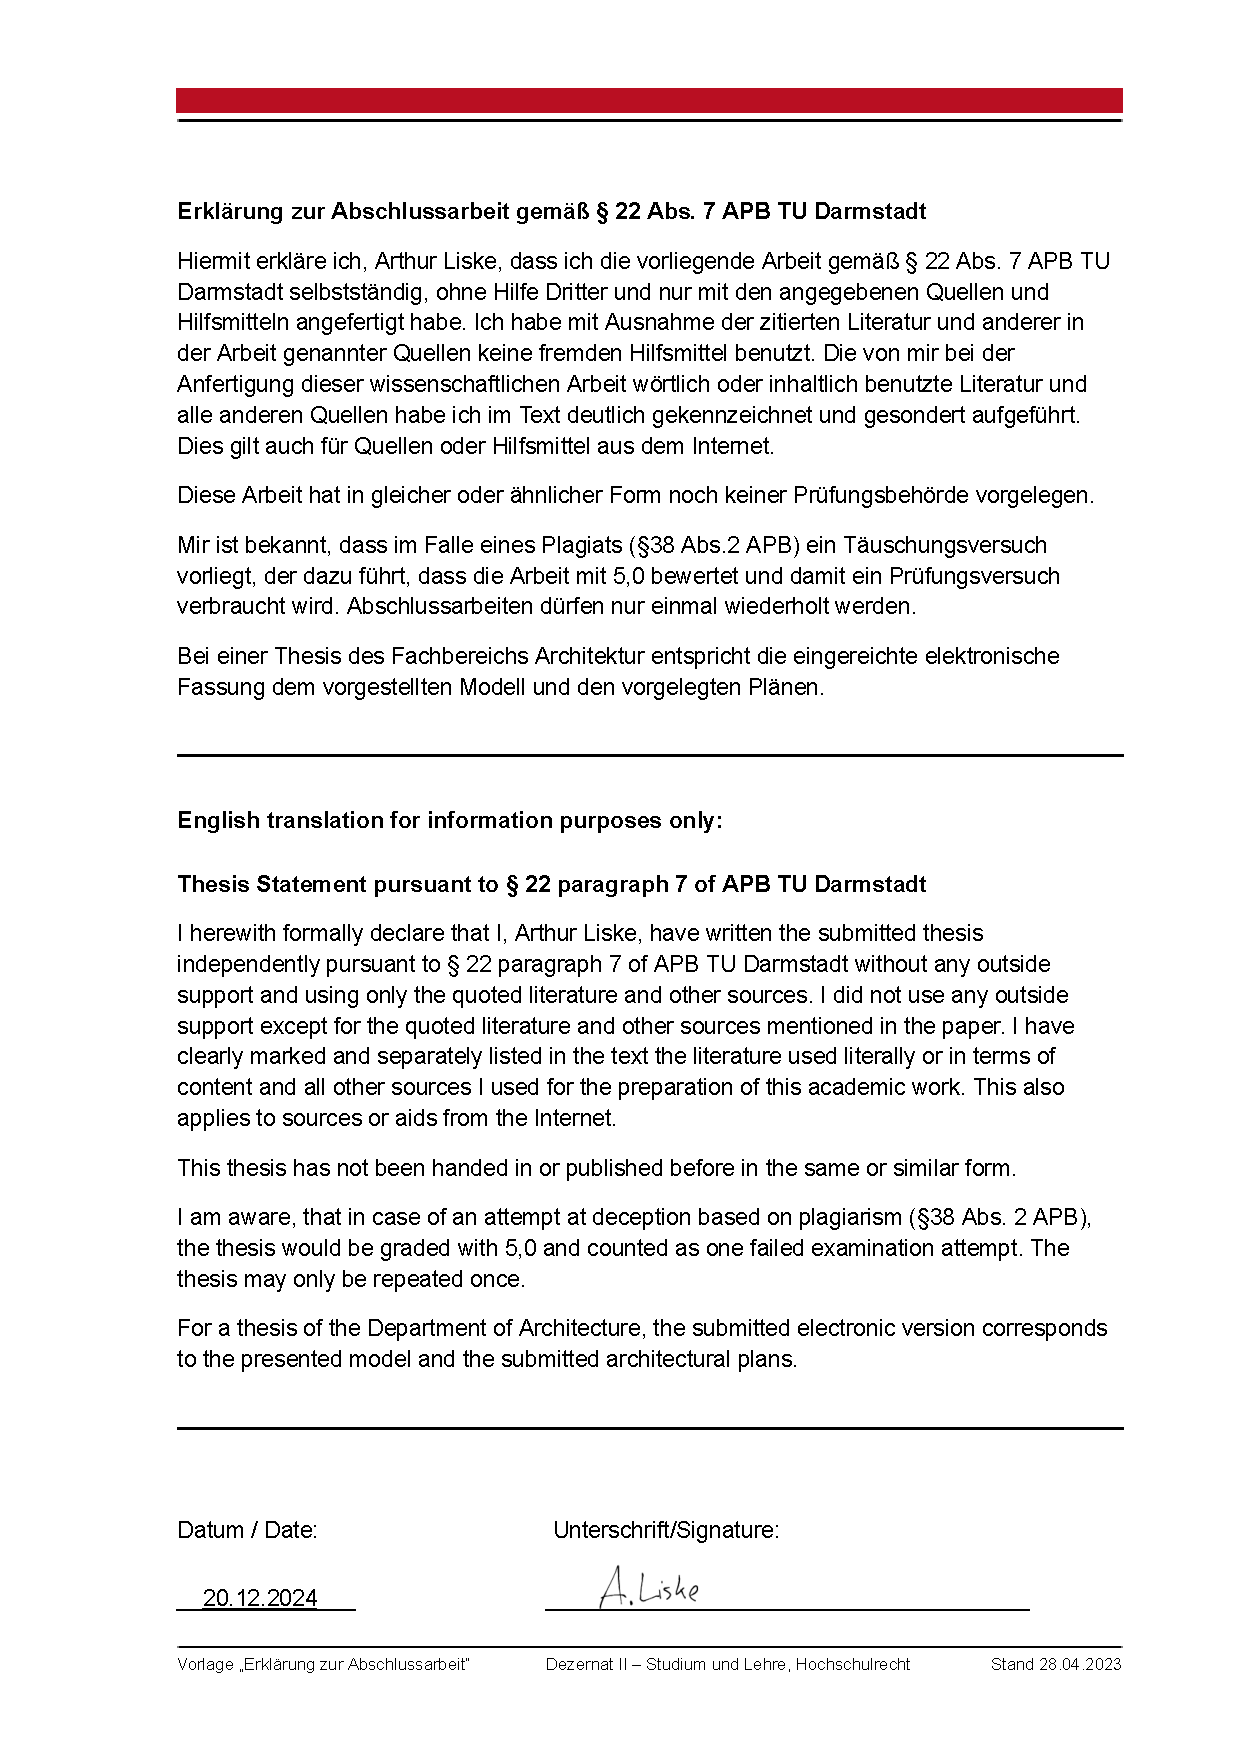
\includepdf{./erklaerung_signed.pdf}

\end{document}
